%%%%%%%%%%%%%%%%%%%%%%%%%%%%%%%%%%%%%%%%%
% Masters/Doctoral Thesis
% LaTeX Template
% Version 1.43 (17/5/14)
%
% This template has been downloaded from:
% http://www.LaTeXTemplates.com
%
% Original authors:
% Steven Gunn
% http://users.ecs.soton.ac.uk/srg/softwaretools/document/templates/
% and
% Sunil Patel
% http://www.sunilpatel.co.uk/thesis-template/
%
% License:
% CC BY-NC-SA 3.0 (http://creativecommons.org/licenses/by-nc-sa/3.0/)
%
% Note:
% Make sure to edit document variables in the Thesis.cls file
%
%%%%%%%%%%%%%%%%%%%%%%%%%%%%%%%%%%%%%%%%%

%----------------------------------------------------------------------------------------
%	PACKAGES AND OTHER DOCUMENT CONFIGURATIONS
%----------------------------------------------------------------------------------------
\documentclass[11pt, oneside]{Thesis} % The default font size and one-sided printing (no margin offsets)

\graphicspath{{Pictures/}} % Specifies the directory where pictures are stored

\usepackage[square,sort,comma,numbers]{natbib} % Use the natbib reference package - read up on this to edit the reference style; if you want text (e.g. Smith et al., 2012) for the in-text references (instead of numbers), remove 'numbers'
\hypersetup{urlcolor=black, colorlinks=false} % Colors hyperlinks in blue - change to black if annoying
\title{\ttitle} % Defines the thesis title - don't touch this

\input{ushyphex}

\usepackage[lining,semibold]{libertine}
\usepackage[T1]{fontenc}
\usepackage{textcomp}
\renewcommand*\ttdefault{txtt}
\usepackage{amsthm}
\usepackage[libertine,cmintegrals,bigdelims,vvarbb]{newtxmath}
\usepackage[scr=rsfso]{mathalfa}
\usepackage{bm}
\useosf

\usepackage[compact]{titlesec}
\usepackage{algorithm}
\usepackage{algpseudocode}
\usepackage{array}
\usepackage{booktabs}
\usepackage{caption}
\usepackage{datetime}
\usepackage{mathtools}
\usepackage{paralist}
\usepackage{pdflscape}
\usepackage{rnamacros}
\usepackage{seqsplit}
\usepackage{silence}
\usepackage{subcaption}
\usepackage{tabularx}
\usepackage{url}
\usepackage{xfrac}
\usepackage{xpatch}

\WarningFilter{latex}{Text page}
\WarningFilter{latex}{Float too large for page by}

\makeatletter
\xpatchcmd{\algorithmic}{\itemsep\z@}{\itemsep=.75ex plus1pt}{}{}

% \def\env@cases{
%   \let\@ifnextchar\new@ifnextchar
%   \left\lbrace
%   \def\arraystretch{.7}
%   \array{@{}l@{\quad}l@{}}
% }
% \makeatother

\begin{document}

\frontmatter % Use roman page numbering style (i, ii, iii, iv...) for the pre-content pages

\setstretch{1.3} % Line spacing of 1.3

% Define the page headers using the FancyHdr package and set up for one-sided printing
\fancyhead{} % Clears all page headers and footers
\rhead{\thepage} % Sets the right side header to show the page number
\lhead{} % Clears the left side page header

\pagestyle{fancy} % Finally, use the "fancy" page style to implement the FancyHdr headers

\newcommand{\HRule}{\rule{\linewidth}{0.25mm}} % New command to make the lines in the title page

% PDF meta-data
\hypersetup{pdftitle={\ttitle}}
\hypersetup{pdfsubject=\subjectname}
\hypersetup{pdfauthor=\authornames}
\hypersetup{pdfkeywords=\keywordnames}

%----------------------------------------------------------------------------------------
%	TITLE PAGE
%----------------------------------------------------------------------------------------
\begin{titlepage}
\begin{center}

\textsc{\LARGE \univname}\\[1.5cm] % University name
\textsc{\Large Doctoral Thesis}\\[0.5cm] % Thesis type

\HRule \\[0.4cm] % Horizontal line
{\large \bfseries \ttitle}\\[0.225cm] % Thesis title
\HRule \\[1.5cm] % Horizontal line

\begin{minipage}{0.4\textwidth}
\begin{flushleft} \large
\emph{Author:}\\
\href{http://www.evansenter.com}{\authornames} % Author name - remove the \href bracket to remove the link
\end{flushleft}
\end{minipage}
\begin{minipage}{0.4\textwidth}
\begin{flushright} \large
\emph{Supervisor:} \\
\href{http://clavius.bc.edu/~clote/}{\supname} % Supervisor name - remove the \href bracket to remove the link
\end{flushright}
\end{minipage}\\[3cm]

\large \textit{A thesis submitted in fulfilment of the requirements\\ for the degree of \degreename}\\[0.3cm] % University requirement text
\textit{in the}\\[0.4cm]
\groupname\\\deptname\\[2cm] % Research group name and department name

{\large \today}\\[4cm] % Date
%\includegraphics{Logo} % University/department logo - uncomment to place it

\vfill

\end{center}
\end{titlepage}

%----------------------------------------------------------------------------------------
%	DECLARATION PAGE
%----------------------------------------------------------------------------------------
\Declaration{

\addtocontents{toc}{\vspace{1em}} % Add a gap in the Contents, for aesthetics

I, \authornames, declare that this thesis titled, `\ttitle' and the work presented in it are my own. I confirm that:

\begin{itemize}
\item This work was done wholly or mainly while in candidature for a research degree at this University.
\item Where any part of this thesis has previously been submitted for a degree or any other qualification at this University or any other institution, this has been clearly stated.
\item Where I have consulted the published work of others, this is always clearly attributed.
\item Where I have quoted from the work of others, the source is always given. With the exception of such quotations, this thesis is entirely my own work.
\item I have acknowledged all main sources of help.
\item Where the thesis is based on work done by myself jointly with others, I have made clear exactly what was done by others and what I have contributed myself.\\
\end{itemize}

Signed:\\
\rule[1em]{25em}{0.5pt} % This prints a line for the signature

Date:\\
\rule[1em]{25em}{0.5pt} % This prints a line to write the date
}

\clearpage % Start a new page

%----------------------------------------------------------------------------------------
%	ACKNOWLEDGEMENTS
%----------------------------------------------------------------------------------------
\setstretch{1.3} % Reset the line-spacing to 1.3 for body text (if it has changed)

\acknowledgements{\addtocontents{toc}{\vspace{1em}} % Add a gap in the Contents, for aesthetics
First and foremost, I would like to thank my advisor, Prof. Peter Clote, for the
countless hours spent explaining the nuances of the computational RNA field.
With all the guidance and support he provided over my graduate school career,
I could not have asked for a better advisor.

Additionally, I'd like to thank my family and friends for their support and
encouragement, and the members of my thesis committee for their insights
along the way.
}
\clearpage % Start a new page

%----------------------------------------------------------------------------------------
%	LIST OF CONTENTS/FIGURES/TABLES PAGES
%----------------------------------------------------------------------------------------
\pagestyle{fancy} % The page style headers have been "empty" all this time, now use the "fancy" headers as defined before to bring them back

\lhead{\emph{Contents}} % Set the left side page header to "Contents"
\tableofcontents % Write out the Table of Contents

\lhead{\emph{List of Figures}} % Set the left side page header to "List of Figures"
\listoffigures % Write out the List of Figures

\lhead{\emph{List of Tables}} % Set the left side page header to "List of Tables"
\listoftables % Write out the List of Tables

%----------------------------------------------------------------------------------------
%	THESIS CONTENT - CHAPTERS
%----------------------------------------------------------------------------------------
% \setstretch{2}
\setstretch{1.3}

\mainmatter % Begin numeric (1,2,3...) page numbering

\pagestyle{fancy} % Return the page headers back to the "fancy" style

\setlength{\abovedisplayskip}{0pt}
\setlength{\abovedisplayshortskip}{0pt}

%!TEX root = ../main.tex

\chapter{Introduction}
\label{ch:intro}

\lhead{Introduction}

Introduced in $1958$, the central dogma of biology has been an excellent model for
the biological flow of information, much as Newtonian classical mechanics stood the
test of time for over $200$ years. But just as Einstein’s revolutionary principle of
relativity has upended our understanding of space in a way unheard of since
Copernicus, recent research has gone to confirm that for all our scientific
progress, the cell still holds fundamental mysteries, and even the central dogma
isn't sacred. Even Francis Crick himself indicated in \citep{crick:1970wb} that
ribonucleic acids (RNAs) likely had a role beyond the traditional {\em messenger}
intermediary between
DNA and proteins, as evidenced by viral RNAs \citep{coffin:1997ws}. Though recent
research continues to suggest that the genome is pervasively transcribed, current
estimates indicate that only 1.2\% of the mammalian genome constitutes
protein-coding sequences \citep{berretta:2009tq,clark:2011cc,jensen:2013vb}. The
study of the transcriptome has led to the identification of a wide variety of
non-coding RNAs (ncRNAs) that highlight the diversity of roles for which RNA can
be put to use \citep{costa:2005ug}. Now understood to be much more than the
intermediary step between DNA and proteins, RNAs have been implicated in a variety
of regulatory and enzymatic activities, including gene knockdown and silencing
\citep{fire:1998tv,mccaffrey:2002tf,hannon:2002vn,he:2004uk},
transcriptional and translational regulation \citep{nudler:2004vm,mandal:2004vh},
intronic splicing \citep{kruger:1982wk,cech:1990tn}, cite-specific cleavage
\citep{doherty:2001wq}, and more.
A prevailing theory now suggests that self-replicating RNA molecules were the
predecessors to all life on Earth---the RNA world hypothesis \citep{gilbert:1986td}.
As our appreciation of RNA diversity has increased,
significant effort has been put forth by the scientific community to understand
and characterize the properties of these molecules.

Unlike DNA, RNA is generally single stranded and thus able to interact with itself
to form interesting shapes with various functional characteristics, akin to
proteins. RNA is a polymer comprised of four monomer {\em building blocks}:
the purines
adenine (A) and guanine (G); and the pyrimidines cytosine (C) and uracil (U). These
nucleotides can form planar base pairs comprised of energetically favorable
hydrogen bonds, the stacking of which produces a stable {\em helix} structure
\citep{yakovchuk:2006bm}. There are only a select set of possible base pairs; the
Watson-Crick pairs (A-U, G-C) or the G-U wobble pair. Given an arbitrary RNA
sequence $\seq = \seqN$, where $s_i \in \{\text{A,\,U,\,G,\,C}\}$, we can define
a secondary structure \str for \seq as the set of index tuples indicating those
bases involved in a base pair within \seq. Again like proteins, RNA molecules tend
to fold into a `native' conformation, usually that which minimizes free energy.
While protein folding is predominantly motivated by hydrophobic
interactions, RNA structure is driven by stacking base pair interactions, and
therefore secondary structure tends to be a much better predictor for the function
of the molecule in question than is the case with proteins, whose function is
largely determined by 3D `tertiary' structure.

From a computational perspective, the history of RNA folding is far too long for
proper treatment within this introduction. Instead we will touch upon just some
of the major milestones to get a flavor for what progress has been made. In $1978$,
Michael Waterman presented the first graph-theoretic model of single stranded
nucleic acids such as RNA \citep{waterman:1978va}. This was followed in $1980$ by
the work of Ruth Nussinov and Ann Jacobson, who together presented an algorithm for
determining the maximally matching secondary structure \str for
a given RNA sequence \citep{nussinov1980}, using dynamic programming
\citep{bellman:1952vza}. In the following years Michael Zuker and Patrick Stiegler
developed an algorithm and accompanying software for the \mfe
formulation of the problem \citep{zuker:1981tf,zuker:1989im}. In $1990$, John
McCaskill showed how dynamic programming could be used to compute the
partition function for an RNA molecule, and even compute the probability that an
arbitrary base is bound \citep{mccaskill}. Alongside these early developments,
more robust energy models were experimentally derived \citep{turner,turner:2009vy},
further improving the accuracy of computational models.

Fast-forwarding to today, there is now a huge collection of software aimed at
computing various properties of RNAs, be it folding, inverse folding, kinetics,
design, and more. The work that we present here intends to be a contribution
to the diverse toolset that researchers have at their disposal for the analysis
and design of both existing and novel RNA sequences.

\section{Thesis Content}
\label{sec:intro:thesiscontent}

The work of this thesis is based on the following four journal articles, alongside
unpublished data and observations. The journal articles constituting the
primary body of research include:

\begin{itemize}
\setstretch{1.3}
\item Senter, E., Sheikh, S., Dotu, I., Ponty, Y., \& Clote, P. (2012). Using the Fast Fourier Transform to Accelerate the Computational Search for RNA Conformational Switches. PloS One, 7(12), e50506. \url{http://doi.org/10.1371/journal.pone.0050506}
\item Ding, Y., Lorenz, W. A., Dotu, I., Senter, E., \& Clote, P. (2014). Computing the Probability of RNA Hairpin and Multiloop Formation. Journal of Computational Biology : a Journal of Computational Molecular Cell Biology, 21(3), 201–218. \url{http://doi.org/10.1089/cmb.2013.0148}
\item Senter, E., Dotu, I., \& Clote, P. (2014). RNA folding pathways and kinetics using \twoD energy landscapes. Journal of Mathematical Biology, 70(1-2), 173–196. \url{http://doi.org/10.1007/s00285-014-0760-4}
\item Senter, E., \& Clote, P. (2015). Fast, Approximate Kinetics of RNA Folding. Journal of Computational Biology : a Journal of Computational Molecular Cell Biology, 22(2), 124–144. \url{http://doi.org/10.1089/cmb.2014.0193}
\end{itemize}

Text, figures, and tables from these papers are used throughout this thesis without
additional notice.

\section{Thesis Organization}
\label{sec:intro:thesisorg}

The remainder of this thesis is organized in the following fashion. We begin in
\Chref{rfinder} with the presentation of \rfinder, a pipeline of
software intended to facilitate the detection of full \rb sequences
alongside their corresponding `on' and `off' structures in genomic data. In
\Chref{fftbor} we introduce the program \fftbor, which computes---for
each integer $k$---the Boltzmann probability \pk of the subensemble of structures
whose \bpd to an input reference structure \str is $k$.
In \Chref{ffttwo} we extend this idea to simultaneously consider two
reference structures \strST and produce as a result the coarse-grained \twoD energy
landscape where---for each integer pair $x,y$---we compute the Boltzmann
probability $p_{x,y}$
of those structures whose \bpd from \strS [resp. \strTresp] is $x$
[resp. $y$]. This program---\ffttwo---allows for the efficient approximation of
kinetic characteristics of RNA molecules, presented in \Chref{hermes}
through the software package \hermes. Finally in \Chref{disc} we conclude
with a summary of this work as a whole, and consider its place in the greater
ecosystem of computational RNA tools.


%!TEX root = ../main.tex

\newcommand{\fnaRetrievalTime}{\formatdate{25}{11}{2014} at \formattime{9}{14}{0}}

\chapter{Ribofinder}
\label{ch:rfinder}

\lhead{Ribofinder: A \Rb Detection Pipeline}

\section{Introduction}
\label{sec:rfinder:intro}

In this chapter, we present the \rfinder program---a pipeline to facilitate the
detection of putative \grbs across genomic data. The \rfinder
tool operates in three stages. First we use \infernal \cite{infernal} and \tthp \cite{ermolaeva:2000cl} to detect
putative aptamers and expression platforms, two distinct components of
\rbs described in section \ref{sec:rfinder:bkgrnd}. After coalescing
this data into a pool of candidate \rbs, we use \rfold \cite{lorenz.amb11} with constraints
based on experimental data to compute the two distinct structural
conformations---`gene on' and `gene off'. In the third and final stage, we
leverage \foldalign \cite{havgaard:2007ca} to measure the similarity between our candidate pool and a
canonical \grb well studied in the literature, the
xanthine phosphoribosyltransferase (xpt) \grb from {\em Bacillus subtilis}. At the time
of this writing, Prof. Dr. Mario
M\"orl at Universit\"at Leipzig is overseeing preliminary structural
validation of predicted gene on and off structures for a number of
computationally predicted \grbs in {\em B. megaterium}.

\subsection{Organization}
\label{subsec:rfinder:org}

This chapter is organized in the following fashion. After providing background
on the structural components of a \rb alongside their biological
significance, we outline the deficiencies in the `state of the art' software
when as it relates specifically to \rb detection. We then move on to outline
the three stages of \rfinder: candidate selection, structural prediction, and
candidate curation. Having described the approach of the software, we move on
to present our findings in using \rfinder to detect \grbs across
the bacterial RefSeq database. Finally, we provide brief commentary on possible
extensions of the algorithm to locate other flavors of \rbs, of which
adenine-sensitive aptamers are a straightforward extension.

\section{Background}
\label{sec:rfinder:bkgrnd}

Riboswitches are regulatory mRNA elements that modulate gene expression via
structural changes induced by the direct sensing of a small-molecule metabolite.
Most often found in bacteria, riboswitches regulate diverse pathways including the
metabolism and transport of purines, methionine, and thiamin amongst others. The
structure of a riboswitch includes an aptamer domain---involved in the direct
sensing of the small-molecule---and a downstream expression platform whose
structure changes upon the aptamer binding the metabolite. Because of the
discriminatory nature of metabolite sensing, groups have had great success in
finding representative examples of aptamers across a diverse collection of
bacterial species; RFam 12.0 currently contains 26 different families of aptamers
involved in different metabolic pathways. Whereas there exists strong sequence and
structural similarity within the aptamer of a riboswitch family, the expression
platform is highly variable, and thus challenging to capture using traditional
SCFG-based approaches. For this reason databases such as RFam only contain the aptamer
portion of the riboswitch, and there exists no database providing sequences
including expression platforms, necessary for capturing the `on' and `off'
conformations of this regulatory element. We have developed a new pipeline---
called \rfinder---which can detect putative riboswitches including their
expression platforms and likely conformational structures across a wide collection
of genomic sequences.

\section{The \rfinder pipeline}
\label{sec:rfinder:pipeline}

At the time of our retrieval (\fnaRetrievalTime), the RefSeq database hosted by
NCBI comprised 5,121 complete bacterial genomes with corresponding genomic
annotations. In order to both detect putative full riboswitches across this
collection of data as well as filter the candidates down to a number tractable for
experimental validation, we developed a novel pipeline which takes a three-tiered
approach to candidate selection. Our approach is to
\begin{inparaenum}[\em 1\upshape)]
\item identify a pool of candidate riboswitches across genomic data;
\item perform a coarse-grained filtering of the candidate pool based on structural
characteristics; and finally
\item fine-grained curation of the candidates based on a collection of measures
and pairwise similarity.
\end{inparaenum} Figure \ref{fig:rfinder:flowchart} outlines this approach as a
flowchart.

\begin{figure}[!ht]
\centering
\includegraphics[width=.9\textwidth]{Figures/Ribofinder/ribofinderOverview.pdf}
\caption{Outline of the approach for the \rfinder pipeline.}
\label{fig:rfinder:flowchart}
\end{figure}

In the following discussion, we describe the application of \rfinder to identify unannotated guanine purine riboswitches; guanine-sensing cis-regulatory elements which modulate the expression of genes involved in purine biosynthesis.

\subsection{Step 1: Candidate selection}
\label{subsec:rfinder:selection}

The RefSeq data we used for analysis contains 5,121 annotated bacterial genomes across 2,732 different organisms, totaling over $9.5 * 10^9$ bases. We used the program \infernal to determine the coordinates of putative aptamer structures within the RefSeq genomes, and \tthp to locate candidate rho-independent transcription terminators.

\subsubsection{Detecting Aptamers with \infernal}
\label{subsubsec:rfinder:infernal}

\infernal \cite{infernal} uses a stochastic context-free grammar (SCFG) with a user-provided multiple sequence alignment (MSA) to efficiently scan genomic data for RNA homologs, taking into consideration both sequence and structural conservation. Using the purine aptamer MSA from RFam 12.0 (RF00167), \infernal (v1.1.1, default options) detects 1,537 significant hits having E-value $<= 0.01$. Because \infernal leverages the concept of a `local end'---a large insertion or deletion in the alignment at reduced cost---it is possible for the software to return a significant hit whose aligned structure does not have the canonical three-way junction observed in all purine riboswitches. \rfinder prunes these truncated \infernal hits by converting the alignment structure into a parse tree, and only permitting trees of sufficient complexity to contain a multiloop (described further in \ref{subsubsec:rfinder:shapes}). The pyrimidine residue abutted next to the P1 stem in the J3--1 junction differentiates between guanine and adenine-sensing riboswitches by binding the complimentary purine ligand; for our interest in \grbs exclusively we require the presence of a cytosine at this residue. In total, using \infernal with these additional filters yields 1,280 guanine aptamers across 555 unique organisms (note: here and elsewhere I define a `unique organism' as having a unique taxonomy ID).

\subsubsection{Detecting Expression Platforms with \tthp}
\label{subsubsec:rfinder:tthp}

\tthp \cite{ermolaeva:2000cl} detects rho-independent terminators in bacterial genomes in a context-sensitive fashion by leveraging the protein annotations available in PTT data. These terminator sequences canonically have a stable hairpin loop structure immediately preceding a run of $5+$ uracil residues, the combination of which causes the ribosomal machinery to stall and dissociate from the transcript. \tthp performs a genomic scan to determine candidate loci with this motif, and returns scored hits. The scoring system considers both structural homology and the genomic contextual information available in the PTT file. Across our collection of bacterial genomes acquired from NCBI RefSeq data, \tthp identified 2,752,469 rho-independent terminators using the default filters.

Due to the spatially-mediated structural regulation of purine riboswitches, whereby ligand interaction with the aptamer domain induces local structural rearrangement in the expression platform, we paired aptamers with corresponding terminators by minimizing the genomic distance, with an upper bound of 200 nucleotides between the end of the aptamer domain and start of the terminator. This approach yields 577 candidate riboswitches, 81 of which have multiple rho-independent terminators within range of a putative aptamer produced by \infernal. For these, we simply pair the closest \tthp hit with the aptamer domain.

\begin{figure}[!ht]
\centering
\includegraphics[width=.9\textwidth]{Figures/Ribofinder/refseqGenomeSizes.pdf}
\caption{Histogram displaying the distribution of genome sizes across the RefSeq
data analyzed, comprising 5,172 bacterial genomes. Genome size is shown using a
$\log_{10}$ scale.}
\label{fig:genomeSizes}
\end{figure}

\subsection{Step 2: Structural prediction}
\label{subsec:rfinder:strpred}

Until this point we have been focused on the generation of candidate sequences
from our RefSeq dataset, without yet focusing on the specifics of underlying
secondary structures for these candidates. In the following section, we explain
how constraint folding is used to generate putative `on' and `off' conformations
for each candidate.

\subsubsection{Notation for Representing Abstract RNA Shapes}
\label{subsubsec:rfinder:shapes}

Given an RNA sequence $\seq = \seqN$, where positions $s_i$ are drawn from the collection of single-letter nucleotide codes, i.e.
$s_i \in \{\text{A,\,U,\,G,\,C}\}$, it is possible to describe a corresponding
secondary structure \strS compatible with \seq using the dot-bracket notation.
In this notation, each nucleotide $a_i$ has a corresponding state $s_i$, where
$s_i$ is denoted as a `.' if unpaired and a `(' [resp. `)'] if the left [resp.
right] base in a base pair. Given any two base pairs $(i,j)$ and $(k,l)$ in \strS, then $i < k < j \iff i < l < j$; pseudoknots are not permitted in the structure. A secondary structure taking this form is said to have balanced parentheses, and can additionally be represented using a context-free grammar such as:

\begin{equation} \label{eq:str_cfg}
S \rightarrow S\,.\;|\;.\,S\;|\;(S)\;|\;SS\;|\;\epsilon
\end{equation}

The grammar from \eqref{eq:str_cfg} can be used to generate a parse tree \tree for \strS. The benefit of working with \tree over \strS is that the parse tree offers an abstract representation of secondary structure shape independent of sequence length, permitting us to classify and eventually constrain a large collection of sequences having variable length which are all expected to have the same abstract tree shape. This is analogous to what the Giegerich lab refers to as their `type 5' structural abstraction using the \rshapes tool. Every node in \tree represents a helix in \strS, and internally tracks the indices of both its beginning $(i,j)$ and closing $(k,l)$ base pair. We use a level-order naming convention to refer to helices within the parse tree, whereby a position \treePos{p}{1} references the first child of the root node, \treePos{p}{1,2} references the second child of \textdown{\ms{p}}{1}, and generally \treePos{p}{$i_1,i_2,\cdots,i_n$} refers to the $i_n$\textsuperscript{th} child of \treePos{p}{$i_1,i_2,\cdots,i_{n-1}$}. To reference specific nucleotides in the context of their location relative to a helix, we use the opening and closing base pairs $(i,j)$ and $(k,l)$ as landmarks. Thus, \treeIdx{p}{1}{l} is the index in \strS of the right-hand side closing base pair of \treePos{p}{1}. We use the notation \treePos{t}{$i$} to refer to the subtree of \tree whose root is \treePos{p}{$i$}.

Finally, we introduce the concept of a tree signature. The tree signature for a tree \tree is a list of the node depths when traversed in a depth-first pre-order fashion. To provide a concrete example, consider the following experimentally validated xpt \grb from Bacillus subtilis subsp. subtilis str. 168 (NC\_000964.3 2320197--2320054) with corresponding gene off structure as seen in Figure \ref{fig:rfinder:xptOff}.
\medskip

\begin{figure}[!ht]
\centering
\begin{subfigure}[h]{\textwidth}
\centering
\includegraphics[width=.9\textwidth]{Figures/Ribofinder/NC_000964_3_2320197_2320054_OFF.pdf}
\end{subfigure} \\
\medskip
\begin{subfigure}[h]{\textwidth}
\centering
\includegraphics[width=.9\textwidth]{Figures/Ribofinder/NC_000964_3_2320197_2320054_ON.pdf}
\end{subfigure}
\caption{{\em (Top)} The xanthine phosphoribosyltransferase (xpt) \grb from
{\em B. subtilis} subsp. subtilis str. 168 (NC\_000964.3 2320197--2320054),
and corresponding gene off structure derived from crystallography analysis in
complex with guanine \cite{breaker:riboswitch2}. {\em (Bottom)} The experimentally
derived gene on structure for \Bsxpt.}
\label{fig:rfinder:xptOff}
\end{figure}

The \rshapes `type 5' representation for this structure is \ms{[[][]][][]} (note the coalesced left bulge in the hairpin immediately downstream the closing multiloop stem, at helix \treePos{p}{2}) and the tree signature for this parse tree of the structure is \ms{[0,1,2,2,1,1]}.

We leverage the notion of abstract structural filtering initially to ensure that all \infernal aptamer hits have a tree signature of \ms{[0,1,2,2]}, which represents a three-way junction, and that the binding site for the guanine ligand $\treeIdx{p}{1}{l - 1} = \text{C}$. These filters, in combination with the proximal terminator hairpins produced by \tthp yield the aforementioned 577 candidate \grbs for which we then try to produce reasonable gene on and off structures.

\subsubsection{Constrained Folding to Predict Switch Structures}
\label{subsubsec:rfinder:consfold}

To restrict our search to unannotated \grbs, and further ensure that we are not re-detecting sequences based off the RFam covariance model provided to \infernal, we constrain our search to those RefSeq organisms not represented in the RFam seed alignment. 503 of the 577 candidates, or 87.18\% represent putative unannotated riboswitches not represented by RF00167.

The gene off structure \strOff for a \grb is the easier of the two to find computationally, since the terminator loop is exceptionally thermodynamically stable. In the gene on conformation \strOn, the P1 stem of the multiloop partially dissociates and an anti-terminator loop forms between the region immediately 3' of the P1 stem and what was the left-hand side of the terminator loop. This truncated P1 stem, which closes the three-way junction in the aptamer, is exceptionally unstable based on present energy models available for structural folding, and requires special treatment to reconstitute in our final structures.

The software \rfold (v2.1.8) allows for the folding of RNA molecules with `loose' constraints. In this model of constrained folding, the resulting structure produced by the software guarantees not to explicitly invalidate any user-provided constraints, but does not guarantee all constraints will be satisfied in the resulting structure. For each of the candidate \grbs, having \treeFor{\infernal} and \treeFor{\tthp}, we build the following constraint masks:

\begin{center}
\begin{tabularx}{\linewidth}{*{2}{L}}
  \toprule
  Guanine gene off constraint mask & Guanine gene on constraint mask \\
  \cmidrule(lr){1-2}
  \multicolumn{2}{l}{Prohibit base pairing upstream of \treeIdx{p}{1}{i} and
  downstream of \treeIdx{p}{2}{l}.} \\
  \multicolumn{2}{l}{Force base pairs and unpaired regions in \treePos{t}{1}, with
  the exception of \treePos{p}{1}.} \\
  \multicolumn{2}{l}{Prohibit formation of \treePos{p}{1} stem, which closes the
  three-way junction.} \\
  \cmidrule(lr){1-2}
  Force base pairs and unpaired regions in \treePos{t}{2}. &
  Require $m$ nucleotides starting from \treeIdx{p}{1}{l + 3} to pair to the
  right, where $m = len(\treePos{p}{2})$, and require the left-hand side of the
  \treePos{p}{2} helix to pair to the left. \\
  & Disallow pairing downstream of \treeIdx{p}{2}{j}. \\
  \bottomrule
\end{tabularx}
\end{center}

These constraint masks are run using the command-line flags \ms{-d 0 -P rna\_turner1999.par} to disable dangles and use the Turner 1999 energies respectively. Experimental evidence using inline probing suggests that the `on' conformation of the \grb has a reduced P1 stem length of 3 base pairs; in practice we were unable to force \rfold to respect this constraint regardless of command-line options specified. For this reason we reconstitute the P1 stem in both structures after constrained folding, having length equivalent to it the \infernal P1 stem (resp. 3 base pairs) in the gene off (resp. gene on) structure.

This difficulty with \rfold can be shown by using the constraint-produced structures as exhaustive constraints themselves. All unpaired nucleotides in \strOff and \strOn are notated by a `\ms{x}' and all base pairs by `\ms{()}' for the 5' and 3' side of the pair respectively to form new constraints mask \strConst{off} and \strConst{on}, having all bases' state explicitly specified. By refolding all 577 candidate sequences with \strConst{off} and \strConst{on} using the same options as before, only 463 (or 80.24\%) of the resulting structures from \strConst{off} have the tree signature prefix \ms{[0,1,2,2,1]}, and just 21 (or 3.64\%) of the \strConst{on} structures correctly re-fold their multiloop.

\begin{figure}[!ht]
\centering
\begin{subfigure}[h]{\textwidth}
\centering
\includegraphics[width=.9\textwidth]{Figures/Ribofinder/NC_014019_1_1427313_1427501_OFF.pdf}
\end{subfigure} \\
\medskip
\begin{subfigure}[h]{\textwidth}
\centering
\includegraphics[width=.9\textwidth]{Figures/Ribofinder/NC_014019_1_1427313_1427501_ON.pdf}
\end{subfigure}
\caption{{\em Top:} the computationally predicted gene off conformation of sequence NC\_014019.1 1427313--1427501, using \rfold from the ViennaRNA 2.1.8 suite, with dangles disabled and the Turner 1999 energies. This sequence is located upstream of the xpt gene in {\em B. megaterium} QM B1551. {\em Bottom:} the gene on conformation.}
\label{fig:example_ss}
\end{figure}

\subsection{Step 3: Candidate curation}
\label{subsec:rfinder:curation}

Until now, we have described our approach for generating the 503 \grb candidates
in RefSeq, alongside their gene on and off structures. Unfortunately the
experimental validation of all 503 candidates is not tractable, so it was
necessary to reduce this collection again to a more manageable size, while only
keeping the most promising candidates. Our original approach involved using
\foldalign alongside the \ms{needleall} tool from XXX \cite{xxx}, to simultaneously
select sequences which closely approximate the more thermodynamically stable
gene off conformation of the experimentally known \Bsxpt \grb, while minimizing
sequence similarity between candidates selected for experimental validation. Due to
experimental constraints, we elected finally to instead choose a small number
($n = 2$) of organisms easily available which had multiple promising hits as our
experimental candidate pool.

\section{Using \rfinder against the RefSeq database}
\label{sec:rfinder:refseq}

\section{Extending beyond \grbs}
\label{sec:rfinder:ext}

%!TEX root = ../main.tex

\chapter{FFTbor}
\label{ch:fftbor}

\lhead{FFTbor}

\section{Introduction}
\label{sec:fftbor:intro}

In this chapter, we present the \fftbor algorithm and accompanying software.
\fftbor is a novel algorithm developed with the intent of efficiently computing
the Boltzmann probability of those structures whom, for a given input RNA
sequence \seq, differ by $k$ base pairs. By leveraging polynomial interpolation
via the \fft, this algorithm runs in \On{4} time and
\On{2} space, a significant improvement over its predecessor. The accompanying
software which implements this algorithm has been used to predict the location
of expression platforms for putative \rbs in genomic data, and to
evaluate the correlation between kinetic folding speed and landscape ruggedness.

\subsection{Organization}
\label{subsec:fftbor:org}

This chapter is organized in the following fashion. First, we provide
background on
the problem which \fftbor aims to address, as well as a brief overview of
existing approaches. We follow by a formal explanation of the problem, and
proceed to describe how the energy landscape is coarsified into discrete bins.
We then develop the recursions for the parameterized partition function using
the Nussinov-Jacobson energy model, which allows us to exposé the novel aspects
of the algorithm. After developing the recursions, we indicate how they can be
reformulated as a polynomial whose coefficients $c_k=\bfZ{k}{1,n}$. We then
describe how the \fft can be employed to efficiently compute the coefficients
$c_k$, finishing our description of the underlying algorithm. Then we proceed
to present two applications of \fftbor, an application to RNA kinetics and
another to \rb detection in genomic data. Finally, we give reference
to the full recursions using the more accurate Turner energy model, which the
underlying implementation actually uses.

\section{Background}
\label{sec:fftbor:bkgrnd}

\section{Formalization of the problem}
\label{sec:fftbor:formal}

\fftbor aims to compute the coefficients $p_0,\dots,p_{n-1}$ of the polynomial

\begin{align}
\label{eq:fftbor:pOfX}
p(x) = p_0 + p_1 x + p_2 x^2 + \dots + p_{n-1} x^{n-1},
\end{align}

where $p_k$ is defined as $p_k = \frac{Z_k}{Z}$. We employ the \fft to compute
the \idft on values $y_0,\dots,y_{n-1}$, where
$y_k = p(\omega^k)$ and $\omega = e^{2 \pi i/n}$ is the principal $n$th complex
root of unity and $p(x)$ is defined in
equation~(\ref{eq:fftbor:pOfX}). By leveraging
complex
roots of unity in conjunction with the \idft the we subvert numeric instability
issues observed with both Lagrange interpolation and Gaussian elimination.

Consider an RNA sequence $\seq = \seqN$, where
$s_i \in \{\text{A,\,U,\,G,\,C}\}$, i.e. a sequence of nucleotides. We can describe a
secondary structure \str which is compatible with \seq as a collection of
base pair tuples $(i,j)$, where $1 \le i \le i+\theta < j \le n$ and
$\theta \ge 0$ (generally taken to be 3), the minimum number of unpaired bases
in a hairpin loop due to steric constraints.

To more simply develop the underlying recursions for \fftbor, we introduce a
number of constraints on the base pairs within \str. Firstly, we require that
each base pair is either a Watson-Crick or G-U wobble, i.e. base pair $(i,j)$
for sequence \seq has corresponding nucleotides $(s_i,s_j)$, which are
restricted to the set

\begin{align}
\label{eq:fftbor:validBP}
\bpSet =
\{\text{(A,\,U),\,(U,\,A),\,(G,\,C),\,(C,\,G),\,(G,\,U),\,(U,\,G)}\}.
\end{align}

With
this constraint satisfied we say that \str is {\em compatible} with \seq, and
for the remainder of this chapter will only consider those structures which are
compatible with \seq.
Secondly, we insist that given two base pairs $(i,j), (x,y)$ from \str,
$i=x \iff j=y$ (bases have at most one partner). Finally, we require that
$i<x<j \iff i<y<j$ (no pseudoknots are allowed). While pseudoknots have been
shown to be present in some biologically relevant RNAs, their inclusion greatly
complicates the recursive decomposition of the structure, and thus it is common
to ignore them.

Provided two secondary structures $\str,\strT$, we can define a notion of
distance between them. There are a number of different definitions of distance
used across the literature; we will use {\em \bpd} for \fftbor.
Base pair distance is defined as the symmetric difference between the sets
\str,\,\strT

\begin{align}
\label{eq:fftbor:dBP}
\dBP{\str}{\strT} = |\str \cup \strT| - |\str \cap \strT|.
\end{align}

Given this definition of distance, two structures \str and \strT are said to
be \kNbrs if $\dBP{\str}{\strT} = k$. It is important to note that
the notion of \bpd is also applicable to restrictions of secondary structures
on the subsequence $\seq_{i,j}$,
i.e. $\str_{[i,j]} = \{ (x,y) \,:\, i \leq  x < y \leq j,  (x,y) \in \str \}$.

For a restriction of base pairs for a given structure $\str_{[i,j]}$,
$\strT_{[i,j]}$ is said to be a \kNbr of $\str_{[i,j]}$ if

\begin{align}
\label{eq:fftbor:dBPonRestriction}
\dBP{\str_{[i,j]}}{\strT_{[i,j]}} =
|\{ (x,y): i \leq x<y\leq j,
(x,y) \in \str - \strT \text{or} (x,y) \in \strT - \str \}| = k.
\end{align}

\section{Derivation of the \fftbor algorithm}
\label{sec:fftbor:math}

Given an RNA sequence $\seq=\seqN$ and compatible secondary structure
\strSt, let \bfZ{k}{} denote the sum of the Boltzmann factors
\boltzf{\str} of all \kNbrs \str of \strSt; i.e.

\begin{align}
\bfZ{k}{} = \bfZ{k}{1,n} =
\sum_{\mathclap{\substack{\str \text{ such that } \\ \dBP{\str}{\strSt}=k}}}\;
\boltzF{\str}
\end{align}

where $E(\str)$ denotes the Turner (nearest neighbor)
energy \cite{}
of \str, $R = 0.00198$ kcal/mol denotes the universal
gas constant and $T$ denotes absolute temperature. From this, it follows that
the full partition function is defined as

\begin{align}
\label{eq:fftbor:partFunc}
\bfZ{}{} = \bfZ{}{1,n} = \sum_{k=0}^n \bfZ{k}{1,n}
\end{align}

since the \bpd between \strSt and \str is at most

\begin{align}
\label{eq:fftbor:maxDist}
\dBP{\strSt}{\str} \leq |\strSt| + \lfloor \frac{n-\theta}{2} \rfloor \leq n.
\end{align}

We can then define the Boltzmann probability of all \kNbrs of \strSt as

\begin{align}
\label{eq:fftbor:probK}
p(k) =\frac{\bfZ{k}{1,n}}{\bfZ{}{1,n}}.
\end{align}

By visualizing the probabilities $p_k$ as a function of $k$, we generate a
coarse grained view of the one-dimensional energy landscape of \seq with
respect to \strSt. When \strSt is taken to be the \mfes for example, one would
anticipate to see a peak at $k=0$, with additional peaks implying additional
metastable structures; local energy minima which could suggest an energetic
trap while folding.

\subsection{Definition of the partition function
\texorpdfstring{\bfZ{k}{1,n}}{}}
\label{subsec:fftbor:recursions}

For the rest of the paper, we consider both \seq as well as the
secondary structure \strSt on \seq to be fixed. We now recall the
recursions from Freyhult et al. \cite{Freyhult.ab05} to determine
the partition function \bfZ{k}{i,j} with
respect to the Nussinov-Jacobson
energy $E_0$ model \cite{nussinovJacobson}, defined by
$-1$ times the number of base pairs; i.e. $E_0(S) = -1 \cdot |S|$.
Although we describe here the recursions for the Nussinov-Jacobson
model, for the sake of
simplicity of exposition, both \rnabor
\cite{Freyhult.ab05} as well as our current software \fftbor,
concern the Turner energy model, consisting of free energy parameters for
stacked bases, hairpins, bulges, internal loops and multiloops.

% The full
% recursions for \fftbor are described for the
% the Turner energy model in the appendix.

The base case for \bfZ{k}{i,j} is given by

\begin{align}
\label{eq:fftbor:initZpart1}
\bfZ{0}{i,j} = 1, \text{ for } i \le j,
\end{align}

since the only $0$-neighbor to a structure \strSt
is the structure \strSt itself, and

\begin{align}
\label{eq:fftbor:initZpart2}
\bfZ{k}{i,j} = 0, \text{ for } k > 0, i \le j \leq i + \theta,
\end{align}

since the empty structure is the only possible structure for a
sequence shorter than $\theta + 2$ nucleotides, and so there are no
\kNbrs for $k>0$. The recursion used to compute
\bfZ{k}{i,j} for $k > 0$ and $j > i+\theta$ is

\begin{align}
\label{eq:fftbor:bfZkij}
\bfZ{k}{i,j} = \bfZ{k-b_0}{i,j-1}\enspace +
\sum_{\substack{(s_r,s_j) \in \bpSet, \\ i \leq r<j}}\qquad
\sum_{\mathclap{w+w'=k-b(r)}}\enspace
\exp(-E_0(r,j)/RT) \cdot \bfZ{w}{i,r-1} \bfZ{w'}{r+1,j-1},
\end{align}

where $E_0(r,j) = -1$ if positions $r,j$ can pair in sequence \seq,
and otherwise $E_0(r,j) = +\infty$. Additionally,
$b_0 = 1$ if $j$ is base-paired
in $\strSt_{[i,j]}$ and $0$ otherwise, and
$b(r)=\dBP{\strSt_{[i,j]}}{\strSt_{[i,r-1]} \cup \strSt_{[r+1,j-1]} \cup\{(r,j)\}}$.
This holds since in a secondary
structure $T_{[i,j]}$ on \seqIJ that is a \kNbr of
$\strSt_{[i,j]}$,
either nucleotide $j$ is unpaired in $[i,j]$ or it is
paired to a nucleotide $r$ such that $i \leq r < j$. In this
latter case it is enough to study the smaller sequence segments
$[i,r-1]$ and $[r+1,j-1]$ noting that, except for $(r,j)$,
base pairs outside of these regions are not allowed, since there
are no pseudoknots. In addition,
for $\dBP{\strSt_{[i,j]}}{T_{[i,j]}} = k$ to hold,
it is necessary for $w+w' = k -b(r)$ to hold, where $w =
\dBP{\strSt_{[i,r-1]}}{T_{[i,r-1]}}$ and $w' =
\dBP{\strSt_{[r+1,j-1]}}{T_{[r+1,j-1]}}$, since $b(r)$ is the
number of base pairs that differ between $\strSt_{[i,j]}$ and a
structure $T_{[i,j]}$, due to the introduction of the base pair
$(r,j)$.

Given RNA sequence \seq and compatible initial structure \strSt,
we define the {\em polynomial}

\begin{align}
\label{eq:fftbor:zOfX}
\emZ{} = \sum_{k=0}^n c_k x^k
\end{align}

where coefficients $c_k=\bfZ{k}{1,n}$. Moreover, because of
(\ref{eq:fftbor:maxDist}) and the fact that the minimum number of
unpaired bases in a hairpin loop $\theta$ is $3$, we know that $c_n=0$,
so that \emZ{} is a polynomial of degree strictly less than $n$.
If we evaluate the polynomial \emZ{} for $n$ distinct values

\begin{align}
\label{eq:fftbor:solutionsForAlpha}
\emZof{}{a_1} = y_1,\dots, \emZof{}{a_n} = y_n,
\end{align}

then the Lagrange polynomial interpolation formula guarantees that
$\emZ{} = \sum_{k=1}^n y_k P_k(x)$, where the polynomials $P_k(x)$ have degree
at most $n-1$ and are given by the Lagrange formula

\begin{align}
\label{eq:fftbor:lagrangeInterpolation}
P_k(x) = \frac{\prod_{i\ne k} (x-x_i)}{\prod_{i \ne k} (x_k-x_i)}.
\end{align}

Since the polynomials $P_k(x)$ can be explicitly computed, it follows that
we can compute the coefficients $c_k$ of polynomial \emZ{}. As we describe
below, the evaluation of \emZ{} for a fixed value of $x$ can be done in
time \On{3} and space \On{2}.  It follows that the coefficients
$c_k=\bfZ{k}{1,n}$ can be computed after
$n$ evaluations of \emZ{}, where the space for each evaluation of \emZ{}
is re-used; hence these evaluations can be performed in time \On{4} and space
\On{2}. Finally,
Lagrange interpolation is clearly computable in time \On{3}.
Although this approach is theoretically sound, there are severe
numerical stability issues related to the interpolation method
\cite{HighamBarycentricInterpolation},
the choice of values $a_1,\dots,a_{n}$ in the interpolation,
and floating point arithmetic (round-off error) related to the
astronomically large values of the partition functions
\bfZ{k}{1,n}, for $0 \leq k < n$. After many unsuccessful
approaches including scaling we obtained excellent results by
interpolating the polynomial $p(x)$, defined in equation (\ref{eq:fftbor:pOfX}),
rather than the polynomial \emZ{}, defined in equation (\ref{eq:fftbor:zOfX}),
and performing interpolation with the Fast Fourier Transform (FFT) \cite{cormen}
where \alphaN are
chosen to be $n$th complex roots of unity,
$\alpha_k = e^{2 \pi i k/n}$.
One
advantage of the FFT is that interpolation can be performed in $O(n \log n)$
time, rather than the cubic time required by using the Lagrange formula
(\ref{eq:fftbor:lagrangeInterpolation}) or by Gaussian elimination. Fewer
numerical operations implies increased numerical stability in our application.

\subsection{Recursions to compute the polynomial
\texorpdfstring{\emZ{i,j}}{}}
\label{subsec:fftbor:polynomial}

Given an initial secondary structure \strSt of a
given RNA sequence \seq, our goal is to compute

\begin{align}
\label{eq:fftbor:defZofK}
\bfZ{k}{1,n} = \sum_{\mathclap{\substack{\str \text{ such that }\\ \dBP{\str}{\strSt}=k}}}\;
\boltzNuss{\str}
\end{align}

where \str can be any structure compatible with \seq.
As previously mentioned, the recurrence relation for \rnabor
with respect to the Nussinov energy model $E_0$ is

% \bfZ{k}{i,j} = \bfZ{k-b_0}{i,j-1}\enspace +
% \sum_{\substack{(s_r,s_j) \in \bpSet, \\ i \leq r<j}}\qquad
% \sum_{\mathclap{w+w'=k-b(r)}}\enspace
% \exp(-E_0(r,j)/RT) \cdot \bfZ{w}{i,r-1} \bfZ{w'}{r+1,j-1},

\begin{align}
\label{eq:fftbor:rnaborNuss}
\bfZ{k}{i,j} = \bfZ{k-b_0}{i,j-1}\enspace +
\sum_{\substack{s_r s_j \in \bpSet, \\ i \le r<j}}
\left(
\boltzNuss{r,j}\enspace \sum_{\mathclap{w+w'=k-b(r)}}\quad
\bfZ{w}{i,r-1} \bfZ{w'}{r+1,j-1}
\right)
\end{align}

where $E_0(r,j)=-1$ if $r$ and $j$ can base-pair and otherwise
$+\infty$, and
$b_0 = 1$ if $j$ is base paired in $\strSt_{[i,j]}$ and $0$ otherwise, and
$b(r)=\dBP{\strSt_{[i,j]}}{\strSt_{[i,r-1]} \cup \strSt_{[r+1,j-1]} \cup\{(r,j)\}}$.
The following theorem shows that an analogous recursion can be used to compute
the {\em polynomial} $\emZ{i,j}$ defined by

\begin{align}
\label{eq:fftbor:polynomialZij}
\emZ{i,j} = \sum_{k=0}^n c_k(i,j)\,x^k
\end{align}

where

\begin{align}
c_k(i,j)\>=\>
\bfZ{k}{i,j}\enspace=\enspace
\sum_{\mathclap{\substack{\str \text{ such that } \\
\dBP{\str}{\strSt_{[i,j]}}=k}}}\enspace
\boltzNuss{\str}.
\end{align}

Here, in the summation, \str runs over structures on \seqIJ, which
are \kNbrs of the restriction $\strSt_{[i,j]}$ of initial structure
\strSt to interval $[i,j]$, and
$E_0(S)=-1 \cdot |S|$ denotes the Nussinov-Jacobson energy of \str.

% \noindent {\sc Theorem 1:} Let \seqN be a given RNA sequence.
\begin{theorem}
Let \seqN be a given RNA sequence.
For any integers $1 \leq i \leq j \leq n$, let

\begin{align}
\emZ{i,j} = \sum_{k=0}^n c_k\,x^k
\end{align}

where

\begin{align}
c_k(i,j) = \bfZ{k}{i,j}.
\end{align}

Then for $i\leq j \leq i+\theta$, $\emZ{i,j}=1$ and for
$j>i+\theta$ we have the recurrence relation

\begin{align}
\label{eq:fftbor:fftborNussPoly}
\emZ{i,j} = \emZ{i,j-1} \cdot x^{b_0} +
\sum_{\substack{s_r s_j \in \bpSet, \\ i\le r<j}}
\left(
\boltzNuss{r,j} \cdot \emZ{i,r-1} \cdot \emZ{r+1,j-1} \cdot x^{b(r)}
\right).
\end{align}

where $b_0 = 1$ if $j$ is base-paired in $\strSt_{[i,j]}$ and $0$ otherwise, and
$b(r) =
\dBP{\strSt_{[i,j]}}{\strSt_{[i,r-1]} \cup \strSt_{[r+1,j-1]} \cup \{(r,j)\}}$.
\end{theorem}

\begin{proof}
First, some notation is necessary.
Recall that if $F$ is an arbitrary
polynomial [resp. analytic] function, then $[x^k] F(x)$
denotes the coefficient of $x^k$ [resp. the $k$th Taylor coefficient in the
Taylor expansion of $F$]. For instance, in equation (\ref{eq:fftbor:pOfX}),
$[x^k]p(x) = p_k$, and in equation (\ref{eq:fftbor:zOfX}),
$[x^k]\emZ{} = c_k(i,j)$.

By definition, it is clear that $\emZ{i,j}=1$ if $i \leq j \leq i + \theta$,
where we recall that $\theta = 3$ is the minimum number of unpaired bases in
a hairpin loop. For $j > i + \theta$, we have

\begin{align}
\begin{split}
[x^k] \emZ{i,j} &= c_k(i,j) = \bfZ{k}{i,j} \\
&= \bfZ{k-b_0}{i,j-1} +
\sum_{r=i}^{j-1}\hspace{2.25em} \sum_{\mathclap{k_0+k_1=k-b(r)}}\enspace
\boltzNuss{r,j} \cdot \bfZ{k_0}{i,r-1} \cdot \bfZ{k_1}{r+1,j-1} \\
&= [x^{k-b_0}] \emZ{i,j-1} \\
&+ \sum_{r=i}^{j-1}\hspace{2.25em} \sum_{\mathclap{k_0+k_1=k-b(r)}}\enspace
\boltzNuss{r,j} \cdot \left\{ [x^{k_0}] \emZ{i,r-1} \right\} \cdot
\left\{ [x^{k_1}] \emZ{r-1,j-1} \right\} \\
&= [x^{k-b_0}] \emZ{i,j-1} \\
&+ \sum_{r=i}^{j-1}\hspace{2.25em} \sum_{\mathclap{k_0+k_1=k-b(r)}}\enspace
\boltzNuss{r,j} \cdot [x^{k_0+k_1}] \emZ{i,r-1} \emZ{r-1,j-1} .\\
\end{split}
\end{align}

By induction, the proof of the theorem now follows.
\end{proof}

Notice that if one were to compute all terms of the polynomial $\emZ{1,n}$
by explicitly performing polynomial multiplications,
then the computation would require \On{5} time and \On{3} space.
Instead of explicitly performing polynomial expansion in {\em variable} $x$,
we instantiate $x$ to a fixed complex number $\alpha \in \mathbb{C}$, and apply
the following recursion for this instantiation:

\begin{align}
\label{eq:fftbor:fftborNussPolyAlpha}
\emZof{i,j}{\alpha} = \emZof{i,j-1}{\alpha} \cdot \alpha^{b_0} +
\sum_{\substack{(s_r,s_j) \in \bpSet, \\ i \le r<j}}
\left(
\boltzNuss{r,j} \cdot
\emZof{i,r-1}{\alpha} \cdot \emZof{r+1,j-1}{\alpha} \cdot \alpha^{b(r)}
\right).
\end{align}

In this fashion, we can compute $\emZof{}{\alpha}=\emZof{1,n}{\alpha}$ in
\On{3} time and \On{2} space. For $n$ distinct complex values
\alphaN, we can compute and save only the
values $\emZof{}{\alpha_0},\dots,\emZof{}{\alpha_{n-1}}$, each time re-using the
\On{2} space for the next computation of $\emZof{}{\alpha_k}$. It follows that
the computation resources used to determine the (column) vector

\begin{align}
\label{eq:fftbor:yColumn}
\bfY = (y_0,\dots,y_{n-1})^{\text T} =
\left(
\begin{array}{l}
y_0 \\
y_1 \\
\vdots \\
y_{n-1} \\
\end{array}
\right)
\end{align}

where
$y_0=\emZof{}{\alpha_0},\dots,y_{n-1}=\emZof{}{\alpha_{n-1}})$ is thus quartic time \On{4} and quadratic space \On{2}.

\subsection{Polynomial interpolation to evaluate
\texorpdfstring{\emZ{i,j}}{}}
\label{subsec:fftbor:fft}

Let $\omega = e^{2 \pi i/n}$ be the principal $n$th complex root of unity.
Recall that the Vandermonde matrix $V_{n}$ is defined to be the
$n \times n$ matrix, whose $i,j$ entry is $\omega^{i \cdot j}$; i.e.

\begin{align}
\label{eq:fftbor:vandermonde}
V_{n} =
\left(
\begin{array}{rrrrr}
1 & 1 & 1 & \dots & 1 \\
1 & \omega & \omega^2 & \dots & \omega^{n-1} \\
1 & \omega^2 & \omega^4 & \dots & \omega^{2(n-1)} \\
1 & \omega^3 & \omega^6 & \dots & \omega^{3(n-1)} \\
\vdots & \vdots & \vdots & \vdots & \vdots \\
1 & \omega^{n-1} & \omega^{2(n-1)} & \dots & \omega^{(n-1)(n-1)} \\
\end{array}
\right)
\end{align}

The Fast Fourier Transform (FFT) is defined to be the $O(n \log n)$
algorithm to compute the Discrete Fourier Transform (DFT), defined
as the matrix product $\bfY = V_{n} {\bf A}$:

\begin{align}
\label{eq:fftbor:dftMatrix}
\left(
\begin{array}{l}
y_0 \\
y_1 \\
y_2 \\
\vdots \\
y_{n-1} \\
\end{array}
\right)
= V_n \cdot
\left(
\begin{array}{l}
a_0 \\
a_1 \\
a_2 \\
\vdots \\
a_{n-1} \\
\end{array}
\right)
\end{align}

On page 837 of \cite{cormen}, it is shown that the
$(i,j)$ entry of $V_n^{-1}$ is $\frac{\omega^{-j i}}{n}$
and that

\begin{align}
\label{eq:fftbor:aFromY}
a_j = \frac{1}{n} \sum_{k=0}^{n-1} y_k\,\omega^{-kj}
\end{align}

for $j=0,\dots,n-1$.

Since we defined \bfY in (\ref{eq:fftbor:yColumn}) by $\bfY =
(y_0,\dots,y_{n-1})^{\text T}$, where
$y_0=\emZof{}{\alpha_0},\dots,y_{n-1}=\emZof{}{\alpha_{n-1}})$
and $\alpha_k = \omega^k e^{2 \pi i k/n}$, it follows that the coefficients
$c_k=\bfZ{k}{1,n}$ in the polynomial
$\emZ{} = c_0 + c_1 x + \dots + c_{n-1} x^{n-1}$ defined in
(\ref{eq:fftbor:zOfX}) can be computed, at least in principle,
by using the FFT. It turns out, however, that the values of
\bfZ{k}{1,n} are so astronomically large, that the ensuing numerical
instability makes even this approach infeasible for values of $n$
that exceed $56$ (data not shown).
Nevertheless, our approach can be modified as follows.
Define \bfY by $\bfY = (y_1,\dots,y_n)^{\text T}$, where
$y_1=\frac{\emZof{}{\alpha_1}}{\emZ{}},\dots,
y_{n}=\frac{\emZof{}{\alpha_n}}{\emZ{}}$, and
\bfZ{}{} is the partition function defined in (\ref{eq:fftbor:partFunc}).
Using the FFT to compute the inverse DFT, it follows from
(\ref{eq:fftbor:aFromY}) that we can compute the probabilities $p_0,\dots,p_{n-1}$
that are coefficients of the polynomial
$p(x) = p_0 + p_1 x + \dots + p_{n-1}x^{n-1}$
defined in equation (\ref{eq:fftbor:pOfX}). For genomics applications, we are
only interested in the $m$ most significant digits of each $p_k$, as described
in the pseudocode that follows.

\begin{algorithm}[H]
\label{algo:fftbor:algo}
\caption{Pseudocode for \fftbor}
\begin{tabular}{ll}
{\sc Purpose:} & Computes the $m$ most significant digits
of probabilities $p_k = \bfZ{k}{1,n} / \bfZ{}{}$ \\
{\sc Input:} & RNA sequence $\seq = \seqN$, secondary
structure \strSt of \seq, integer $m$ \\
{\sc Output:} & Probabilities $p_k = \bfZ{k}{1,n} / \bfZ{}{}$ to $m$ significant digits for $k=0,\dots,n-1$ \\ \hline
\end{tabular}
\begin{algorithmic}[1]
\Procedure{FFTbor}{}
\State $\textit{stringlen} \gets \text{length of }\textit{string}$
\State $i \gets \textit{patlen}$
% \BState \emph{top}:
\If {$i > \textit{stringlen}$} \Return false
\EndIf
\State $j \gets \textit{patlen}$
% \BState \emph{loop}:
\If {$\textit{string}(i) = \textit{path}(j)$}
\State $j \gets j-1$.
\State $i \gets i-1$.
\State \textbf{goto} \emph{loop}.
\State \textbf{close};
\EndIf
\State $i \gets i+\max(\textit{delta}_1(\textit{string}(i)),\textit{delta}_2(j))$.
\State \textbf{goto} \emph{top}.
\EndProcedure
\end{algorithmic}
\end{algorithm}

% \mverbatim
% 1.  generate roots of unity $\omega^k$ for $k=0,\dots,n-1$, where $\omega=\exp(\frac{2 \pi i}{n})$ and $i=\sqrt{-1}$
% 2.  note that the partition function $\bfZ{}{}=y_0=\Z(\omega^0)$
% 3.  for $k=0$ to $n-1$
% 4.    compute $y_k = \Z(\omega^k)$ using recursion (\ref{eqn:RNAborNussRecursionInstantiated})
% 5.    $y_k = 10^m \cdot \frac{y_k}{\bfZ{}{}}$ //normalize $y_k$
% 6.  compute $P = (p_0,\dots,p_{n-1})^{\text T}$ where $p_j =\frac{\sum_{k=0}^{n-1} a_k \omega^{-kj}}{n}$ by using FFT in (\ref{eqn:ajdef})
% 7.  for $k=0$ to $n-1$
% 8.    $p_k = \lfloor 10^m \cdot p_k \rfloor \cdot \frac{1}{10^m}$
% 9.    //truncate to $m$ most significant digits
% |mendverbatim

\section{Benchmarking and performance considerations}
\label{sec:fftbor:benchmarking}

In this subsection, we show that we need only evaluate the polynomial
\emZ{}, as defined in
equation~(\ref{eqn:polynomialYann}), for $n/2$ of the complex $n$th roots
of unity. It is first necessary to recall the definition of complex
conjugate.
Recall that the complex conjugate of $z$ is denoted by $\overline{z}$;
i.e. if $z=\aPbi$ where $a,b \in \mathbb{R}$ are real numbers and
$i = \sqrt{-1}$,  then $\overline{z} = \aMbi$.

\noindent {\sc Lemma 1:} If \emZ{} is the complex polynomial defined in
equation~(\ref{eqn:polynomialYann}), then for any complex $n$th root of
unity $\alpha$, it is the case that $\emZof{}{\overline{\alpha}} =
\overline{\emZof{}{\alpha}}$. In other words, if $\alpha$ is a complex $n$th root
of unity of the form \aPbi, where $a,b \in \mathbb{R}$ and $b>0$, and
if $\emZof{}{\aPbi} = A + Bi$ where $A,B \in \mathbb{R}$, then it is the case that

\begin{align}
\emZof{}{\aMbi} = A - Bi.
\end{align}

\noindent {\sc Proof:} Letting $i = \sqrt{-1}$, if
$\theta = \frac{2 \pi}{n}$, then
$\omega = e^{i \theta} = \cos(\theta) + i \sin(\theta)$
is the principal $n$th complex root of unity, and
$1=\omega^{0},\dots,e^{(n-1)\cdot i \theta}=\omega^{n-1}$ together
constitute the complete collection of all
$n$th complex roots of unity -- i.e. the $n$ unique solutions of
of the equation $x^n -1 = 0$ over the field $\mathbb{C}$ of complex numbers.
Clearly, for any $1 \leq r < n$,
$e^{-i r \theta} = 1 \cdot e^{-i r \theta} =
e^{2 \pi i} \cdot e^{-i r \theta} = e^{i(2 \pi - r \theta)} =
e^{i(n \theta - r \theta)} = e^{i \theta (n - r)}$.
Moreover, if $\omega^r = e^{i r \theta} = a + b i$ where
$b>0$, then we have $e^{-i r \theta} = \aMbi$. It follows that for any
$n$th root of unity of the form \aPbi, where $b>0$, the number \aMbi
is also an $n$th root of unity.

Recall that $\emZ{} = \sum_{k=0}^n c_k x^k$, where
$c_k\in \mathbb{R}$ are real numbers representing the partition function
\bfZ{k}{1,n} over
all secondary structures of a given RNA sequence \seqN,
whose base pair distance from initial structure
\strSt is $k$. Thus, in order to prove the lemma, it suffices to show
that for all values $k=0,\dots,n-1$, if \aPbi is a complex $n$th
root of unity, where $a,b \in \mathbb{R}$
and $b>0$, and if $(\aPbi)^k = C+Di$ where $C,D \in \mathbb{R}$, {\em then}
$(\aMbi)^k = C-Di$. Indeed, we have the following.

\begin{align}
(\aPbi)^m &= \sum_{k=0}^m {m \choose k} a^{m-k}\cdot (bi)^k \\
(bi)^k  &= \left\{
\begin{array}{rl}
b^k &\mbox{if $k \equiv 0 \bmod 4$}\\
i b^k &\mbox{if $k \equiv 1 \bmod 4$}\\
-b^k &\mbox{if $k \equiv 2 \bmod 4$}\\
-i b^k &\mbox{if $k \equiv 3 \bmod 4$}\\
\end{array} \right.
\end{align}

\begin{align}
(\aMbi)^m &= \sum_{k=0}^m {m \choose k} a^{m-k} \cdot (-bi)^k \\
(-bi)^k &= \left\{
\begin{array}{rl}
b^k &\mbox{if $k \equiv 0 \bmod 4$}\\
-ib^k &\mbox{if $k \equiv 1 \bmod 4$}\\
-b^k &\mbox{if $k \equiv 2 \bmod 4$}\\
ib^k &\mbox{if $k \equiv 3 \bmod 4$}\\
\end{array} \right.
\end{align}

It follows that each term of the form
$a^{m-k} \cdot (bi)^k$, for $k=0,\dots,m$, is the complex conjugate of
$a^{m-k} \cdot (-bi)^k$, and thus $(\aPbi)^m$ is the complex conjugate of
$(\aMbi)^m$. Since \emZof{}{\aPbi} is a sum of terms of the form $c_k (\aPbi)^k$,
it follows that \emZof{}{\aMbi} is the complex conjugate of \emZof{}{\aPbi}.
This completes the proof of the lemma. \hfill $\Box$

Lemma 1 immediately entails that we need only evaluate \emZ{} on $n/2$
many of the complex $n$th roots of unity -- namely, those of the form
\aPbi, where $b \geq 0$. The remaining values of \emZ{} are obtained by
taking conplex conjugates of the first $n/2$ values. This, along with a
precomputation of powers of the complex $n$th roots of unity, leads to an
enormous performance speed-up in our implementation of \fftbor.

\section{Coarse-grained kinetics with \fftbor}
\label{sec:fftbor:kinetics}

\section{Riboswitch detection with \fftbor}
\label{sec:fftbor:rb}

%!TEX root = ../main.tex

\chapter{FFTbor2D}
\label{ch:ffttwo}

\lhead{FFTbor2D}

\section{Introduction}
\label{sec:ffttwo:intro}

In this chapter, we present the \ffttwo algorithm and accompanying software.
\ffttwo, like \fftbor described in Chapter \ref{ch:fftbor}, is an algorithm
which computes the paramerized partition function for an input RNA sequence
\seq. \ffttwo computes the two-dimensional coarse energy landscape for \seq
given two compatible input secondary structures \strA and \strB, where position
$(x,y)$ on the discrete energy landscape corresponds to the Boltzmann
probability for those structures \str which have $d_{BP}(\str, \strA)=x$ and
$d_{BP}(\str, \strB)=y$ (where $d_{BP}$ is as defined in equation
\ref{eq:fftbor:dBP}). By again leveraging the \fft, \ffttwo runs in \On{5}
time and only uses \On{2} space---a significant improvement over previous
approaches. This permits the output energy landscape to be used in a
high-throughput fashion to analyze folding kinetics; a topic covered in detail
in Chapter \ref{ch:hermes}.

\subsection{Organization}
\label{subsec:ffttwo:org}

This chapter is organized in the following fashion. Because the history for
this work arises naturally from the background described in section
\ref{sec:fftbor:bkgrnd}, we forego reiteration and instead fall directly into
a technical discussion of the underlying algorithm. We first develop the
recursions for the Nussinov energy model for expository clarity, the
underlying implementation uses the more complicated and robust Turner energy
model. Recursions in place, we then move to show how these lead to
a single variable polynomial $P(x)$ whose coeffecients can be computed by
the \idft, and map to the 2D energy landscape. We describe two exploitations of
$P(x)$, a parity condition and complex conjugates which further reduce the
runtime by a factor of 4. Finally, we contrast this software against \rtwofold,
and outline the performance characteristics of both softwares and highlight
the benefits and drawbacks of both.

\section{Derivation of the \ffttwo algorithm}
\label{sec:ffttwo:math}

\subsection{Definition of the partition function
\texorpdfstring{\bfZ{x,y}{1,n}}{}}
\label{subsec:ffttwo:recursions}

\subsection{Recursions to compute the polynomial
\texorpdfstring{\emZ{i,j}}{}}
\label{subsec:ffttwo:polynomial}

\subsection{Polynomial interpolation to evaluate
\texorpdfstring{\emZ{i,j}}{}}
\label{subsec:ffttwo:fft}

\section{Acceleration of the \ffttwo algorithm}
\label{sec:ffttwo:perf}

\subsection{Optimization due to parity condition}
\label{subsec:ffttwo:parity}

\subsection{Optimization due to complex conjugates}
\label{subsec:ffttwo:compconj}

\section{Benchmarking and performance considerations}
\label{sec:ffttwo:benchmarking}

\section{Applications of the \ffttwo algorithm}
\label{sec:ffttwo:applications}

%!TEX root = ../main.tex

\newcommand{\mathbbP}{\mbox{\bf P}}
\newcommand{\mathbbt}{\mbox{\bf t}}
\newcommand{\mathbbx}{\mbox{\bf x}}

\chapter{Hermes}
\label{ch:hermes}

\lhead{Hermes}

\section{Introduction}
\label{sec:hermes:intro}

In this chapter, we present the \hermes software suite---a collection of
programs aimed at evaluating the kinetic properties of RNA molecules.
Provided a coarse-grained energy landscape generated by \ffttwo (described
in Chapter \ref{ch:ffttwo}), we present software which computes both the \mfpt
and \eqt for this discretized energy landscape. We also provide software which
computes the exact kinetics for an RNA molecule, however since this requires
exhaustive enumeration of all secondary structures---which is known to be an
exponential quantity for the length of the RNA in consideration---the full
kinetics are not expected to be practical for anything beyond a sequence of
trivial length. The software in \hermes presents a practical application of
the energy landscapes computed by the \ffttwo algorithm. Contrasted against
the other kinetics software in the field, \hermes offers similar accuracy
with unparalleled performance which opens up the possibility for large-scale
kinetic analysis {\em in silico}, which we expect to be of use for synthetic
design.

\subsection{Organization}
\label{subsec:hermes:org}

This chapter is organized in the following fashion. We begin by providing
background on the state-of-the-art approaches for kinetic analysis of RNAs.
From there, we move into a technical discussion of two traditional approaches
for kinetics, computation of the \mfpt and the \eqt. With this foundation in
place, we proceed to discuss the high-level organization of the \hermes
software package, and describe in detail each of the four underlying programs
which comprise the kinetics suite. We then move on to present comparitive
benchmarking of \hermes against other methods, before finally concluding with
some remarks on the accuracy and applicability of \hermes to computational
RNA design.

% \section{Background}
% \label{sec:hermes:bkgrnd}

\section{Traditional approaches for kinetics}
\label{sec:hermes:kinetics}

To better understand the underlying algorithms behind the software,
we describe two traditional approaches in kinetics.

\subsection{\Mfpt}
\label{subsec:hermes:mfpt}

Consider a physical process,
which when monitored over time, yields the stochastic sequence
$q_0,q_1,q_2,\dots$ of discrete, observed states. If the transition from
state $q_t$ to $q_{t+1}$ depends only on $q_t$ at time
$t$ and not on the historical sequence of prior states visited,
as often assumed in the case of protein or
RNA folding, then a Markov chain provides a reasonable
mathematical model to simulate the process.

A (first-order, time-homogeneous)
{\em Markov chain} $\mChain = (Q,\pi,P)$ is given by a finite
set $Q = \{ 1,\dots,n \}$ of states, an initial probability distribution
$\pi = (\pi_1,\dots,\pi_n)$, and the $n \times n$
{\em transition probability matrix} $P = (p_{i,j})$.
At time $t=0$, the initial state of the system is
$q_t=i$ with probability $\pi_i$, and at discrete time
$t=1,2,3,\dots$, the system makes a transition from state
$i$ to state $j$ with probability $p_{i,j}$; i.e.
the conditional probability $Pr[ q_{t+1} = j | q_t=i] = p_{i,j}$.
Define the {\em population occupancy frequency} of visiting state
$i$ at time $t$ by $p_{i}(t) = Pr[q_t=i]$.  Denote
$p_{i,j}^{(t)} = Pr[q_t = j | q_0 = i]$ and notice that
the $(i,j)$-th entry of the $t$-th power $P^t$ of matrix $P$  equals
$p_{i,j}^{(t)}$.

The {\em \mfpt} (MFPT) or
{\em \hit} for the Markov chain \mChain,
starting from initial state \xStart and proceeding
to the target state \xEnd, is defined
as the sum, taken over all paths $\rho$
from \xStart to \xEnd, of the path length $\textit{length}(\rho)$
times the probability
of path $\rho$, where $\textit{length}(\rho_0,\dots,\rho_n)$ is defined to
be $n$. In other words,
${\text MFPT} = \sum_{\rho} Pr[\rho] \cdot \textit{length}(\rho)$, where
the sum is taken over sequences $\rho=\rho_0,\dots,\rho_n$ of states
where $\rho_0=\xStart$ and $\rho_n=\xEnd$, and no state is visited more
than once in the path $\rho$.

Given the target state \xEnd, MFPT can be exactly
determined by computing the inverse
$(I - P^{-}_{\xEnd})^{-1}$, where $I$ is the $(n-1)\times (n-1)$ identity
matrix and $P^{-}_{\xEnd}$
denotes the $(n-1)\times (n-1)$ matrix obtained from the
Markov chain transition probability matrix $P$,
by deleting the row and column with index \xEnd.
Letting ${\bf e}$ denote the
$(n-1) \times 1$ column vector consisting entirely of $1$'s, it can be
shown that \mfpt from state \xStart to state \xEnd
is the \xStart-th coordinate
of column vector
$(I - P^{-}_{\xEnd})^{-1} \cdot {\bf e}$ \cite{meyerMFPT}.

The {\em stationary} probability distribution \statDist
is a row vector such that $\pSt \cdot P = \pSt$; i.e.
$\pSt_j = \sum_{i}^n \pSt_i \cdot p_{i,j}$, for all $1\leq j \leq n$.
It can be shown that the stationary probability $\pSt_i$ is the limit,
as $m$ tends to infinity, of the frequency of visiting state $i$ in a
random walk of length $m$ on Markov chain \mChain.
It is well-known that the stationary distribution exists and is unique
for any finite aperiodic irreducible Markov chain \cite{cloteBackofen:book}.

The Metropolis Monte Carlo algorithm \cite{metropolis:MonteCarlo} can
be used to simulate a random walk from initial state \xStart to target state
\xEnd, when energies are associated with the states, as is the case in
macromolecular folding, where free energies can be determined for
protein and RNA conformations from mean field theory, quantum theory,
or experimental measurements. In such cases, a {\em move set}
defines the set $N_x$ of conformations reachable in unit time
from conformation $x$, and the transition probability matrix
$P = (p_{x,y})$ is defined as follows:

\begin{align}
\label{eq:hermes:mfptXitionProb}
p_{x,y} =
\begin{cases}
\frac{1}{|N_x|} \cdot \min\left( 1, \boltzYmX \right)
& \text{if $y \in N_x$} \\
1 - \sum_{k \in N_x} p_{x,k} & \text{if $x=y$} \\
0 & \text{if $y \not\in N_x$, and $x \ne y$} \\
\end{cases}
\end{align}

If $\pSt_x \cdot p_{x,y} = \pSt_y \cdot p_{y,x}$ holds for all distinct
$x,y \in Q$, then
{\em detailed balance} is said to hold, or equivalently the Markov
chain \mChain is said to be {\em reversible}.
If transitional probabilities
are defined as in equation (\ref{eq:hermes:mfptXitionProb}), and if neighborhood
size is constant ($|N_x|=|N_y|$ for all $x,y$), then it is well-known
that the stationary probability distribution
\statDist is the Boltzmann distribution; i.e.

\begin{align}
\label{eq:hermes:stationaryBoltzmannProb}
\pSt_k = \frac{\boltzf{k}}{Z}
\end{align}

where $E(k)$ is the energy of conformation $k$ at temperature $T$,
$R$ is the universal gas constant,
$T$ is absolute temperature, and the {\em partition function}
$Z = \sum_{k=1}^n \boltzf{k}$ is a normalization constant
\cite{waterman:book,cloteBackofen:book}. If neighborhood size is not
constant, as in the case where states are RNA secondary structures and transitions
are restricted to the addition or removal of a single base pair, then
by {\em Hasting's trick}, an equivalent Markov chain can be defined which
satisfies detailed balance -- see equation (\ref{eq:hermes:MFPTwithHastings}).

Following Anfinsen's experimental work on the denaturation and
refolding of bovine pancreatic ribonuclease \cite{anfinsen},
the native conformation is assumed to be the ground state having
minimum free energy. These results justify the use of the Monte Carlo
Algorithm \ref{algo:MonteCarlo} in macromolecular kinetics and
structure prediction.
% \medskip

\begin{figure}[!ht]
\label{fig:hermes:mcmc}
% \hrule \rule[0ex]{0pt}{0pt}
\begin{center}
{\large Pseudocode for the Metropolis Monte Carlo algorithm} \\
\end{center}
\begin{tabular*}{\textwidth}{ll}
{\sc Purpose:} & Compute discrete time $t$ to move from
\xStart to \xEnd, with upper limit of \tMax \rule[-1.5ex]{0pt}{0pt} \\
{\sc Input:} & Starting state \xStart, target state \xEnd and
upper bound on time \tMax \rule[-1.5ex]{0pt}{0pt} \\
{\sc Output:} & Discrete time $t$ taken to reach \xEnd from \xStart
\rule[-1.75em]{0pt}{0pt} \\
\hline \rule[0ex]{0pt}{0pt}
\end{tabular*}
\begin{algorithmic}[1]
\Function{Metropolis}{\xStart, \xEnd, \tMax}
\State $t \gets 0$
\State $x \gets \xStart$
\While{$x \neq \xEnd$ AND $t < \tMax$}
\State $y \in N_x$
\If{$E(y) < E(x)$}
\Comment{Greedy move}
\State $x \gets y$
\Else
\Comment{Metropolis move}
\State $z \in (0,1)$
\If{$z < \boltzYmX$}
\State $x \gets y$
\EndIf
\EndIf
\State $t \gets t+1$
\EndWhile
\State \textbf{return} $t$
\Comment{Return discrete time $t$ to travel from \xStart to \xEnd}
\EndFunction
\rule[-0.35ex]{0pt}{0pt}
\end{algorithmic}
\caption{Caption here}
\end{figure}

The \mfpt from state $x$ to state $y$ can
be approximated by repeated runs of the Monte Carlo algorithm.
In particular, \v{S}ali, Shakhnovich, and Karplus used such Monte Carlo
simulations to investigate the Levinthal paradox of how a protein
can fold to its native state within milliseconds to seconds.
By repeated Monte Carlo simulations using a protein lattice model,
\v{S}ali et al. observed that a large energy difference between
the ground state
and the first misfolded state appears to be correlated with fast folding.

\subsection{\Eqt}
\label{subsec:hermes:eq}

A continuous time {\em Markov process} $\mChain=(Q,\pi,P(t))$
is given by a finite set $Q= \{1,\dots,n\}$ of states, the
initial probability distribution $\pi$,
and the $n\times n$ matrix $P(t)=(p_{i,j}(t))$ of
probability transition functions.

% \footnote{Only in the
% current section does $P(t)$ denote the Markov process
% transition probability matrix.  In all later sections of the paper,
% $P(t) = (P_1(t),\dots,P_n(t))$ will denote the population occupancy
% frequency function, defined in (\ref{eq:hermes:populationOccupancyEquation}).
% In Markov processes, the rate matrix $R$ is used rather than the transition
% probability matrix $P(t)$, so there will be no ambiguity in later
% reserving $P(t)$ to denote the population occupancy function.}

Letting $q_t$ denote the state at (continuous)
time $t$, the probability that the initial state $q_0$ at time $0$ is
$k$ is $\pi_k$, while

\begin{align}
\label{eq:hermes:markovProcess}
p_{i,j}(t) = Pr[q_{t} = j| q_0 = i].
\end{align}

The matrix $P'(t)$ of derivatives, defined by

\begin{align}
  P'(t) = \left(
\begin{array}{ccc}
\frac{d p_{1,1}}{d t}(t) & \dots  & \frac{d p_{1,n}}{d t}(t)\\
\vdots & \ddots & \vdots \\
 \frac{d p_{n,1}}{d t}(t) & \dots  & \frac{d p_{n,n}}{d t}(t)\\
\end{array}
\right),
\end{align}

can be shown to satisfy

\begin{align}
P'(t) = P(t) \cdot R
\end{align}

where $R = (r_{i,j})$ is an $n \times n$ {\em rate matrix} with the
property that each diagonal entry is $-1$ times the row sum

\begin{align}
r_{i,i} = - \sum_{j\ne i} r_{i,j}.
\end{align}

Define the {\em population occupancy} distribution
$p(t) = (p_1(t),\dots,p_n(t))$ by

\begin{align}
\label{eq:hermes:markovProcessPopulationFreq}
p_i(t) = Pr[q(t) = i] = \sum_{k=1}^n\pi_k p_{k,i}(t)
\end{align}

where $q(t)$ denotes the state of the Markov process
at (continuous) time $t$.

In the case of macromolecular folding, where Markov process states
are molecular conformations and conformational energies are available,
it is typical to define the rate matrix
$R = (r_{x,y})$ as follows:

\begin{align}
\label{eq:hermes:eqXitionRate}
r_{x,y} =
\begin{cases}
\min\left( 1, \boltzYmX \right)
& \text{if $y \in N_x$} \\
-\sum_{k \in N_x} p_{x,k} & \text{if $x=y$} \\
0 & \text{if $y \not\in N_x$, and $x \ne y$} \\
\end{cases}
\end{align}

The {\em master equation} is defined by the matrix differential equation

\begin{align}
\label{eq:hermes:masterEquationMatrix}
\frac{d p(t)}{dt} = p(t) \cdot R
\end{align}

or equivalently, for all $1 \leq x \leq n$,

\begin{align}
\label{eq:hermes:masterEquation}
\frac{d p_x(t)}{dt} = \sum_{y=1}^n\, (p_y(t) \cdot r_{y,x} - p_x(t) \cdot
r_{x,y})\; = \sum_{x \ne y}\, (p_y(t) \cdot r_{y,x} - p_x(t) \cdot r_{x,y}).
\end{align}

As in the case of Markov chains,
\statDist is defined to be
the stationary distribution if
$\pSt \cdot P(t)= \pSt$; i.e. $\pSt_k = Pr[ q(0) = k ]$ implies that
$Pr[ q(t) = k] = \pSt_k$ for all $t \in \mathbb{R}$ and
$1 \leq k \leq n$.
Define the {\em equilibrium distribution} \statDist
to be the unique solution for $p(t)$, when the master equation
(\ref{eq:hermes:masterEquation}) is set to equal zero; i.e.

\begin{align}
\label{eq:hermes:equilibriumTime}
\sum_{x \ne y} \pSt_x \cdot r_{x,y} = \sum_{x \ne y} \pSt_y \cdot r_{y,x}.
\end{align}

If the equilibrium distribution exists, then necessarily it is equal to
the stationary distribution. A Markov process is said
to satisfy detailed balance if $\pSt_x \cdot r_{x,y} = \pSt_y \cdot r_{y,x}$,
for all $1 \leq x,y \leq n$, where the rate matrix $R = (r_{x,y})$.

The rate equation $R$ for is usually defined
as in (\ref{eq:hermes:eqXitionRate}) for
Markov processes which model macromolecular folding,
hence it is easy to see that
such Markov processes satisfy detailed balance and moreover that
the equilibrium distribution is the
Boltzmann distribution; i.e.  $\pSt_x = \boltzf{x}$ for
all $1 \leq x \leq n$.
Since detailed balance ensures that the eigenvalues of the rate matrix $R$ are
real, one can solve the matrix differential equation
(\ref{eq:hermes:masterEquation}) by diagonalizing the rate matrix, and thus obtain
the solution

\begin{align}
\label{eq:hermes:populationOccupancyEquation}
p(t) = \sum_{k=1}^n c_k {\bf v}_k e^{\lambda_k t}
\end{align}

where $p(t) = (p_1(t),\dots,p_n(t))$, and the
values $c_k$ are determined by the initial population occupancy
distribution $p(0)$ at time $0$. Here
${\bf v}_k$ denotes the $k$th eigenvector and
$\lambda_k$ the $k$th eigenvalue. In particular,
$c_k = \left(p(0) \cdot T^{-1})\right)_k$, where the $j$-th row of $T$
is the $j$-th left eigenvector of $R$,
and $p(0)$ is the population occupancy distribution
at time $t=0$. If the eigenvalues are labeled in decreasing
order, then $\lambda_1 \geq \lambda_2 \geq \cdots \geq \lambda_n$,
and the largest eigenvalue $\lambda_1=0$ has eigenvector \pSt, corresponding
to the equilibrium population occupancy distribution, which in this case
is the Boltzmann distribution. The
remaining $n-1$ eigenvalues are negative, and their corresponding eigenvectors
correspond to nonequilibrium kinetic {\em relaxation modes}.

In our software \hermes, we prefer to work with column vectors and
right eigenvectors due to our usage of the GSL scientific computing library,
and so the population occupancy frequency
$p(t)$ is defined to be the column vector
$p(t)=(p_1(t),\dots,p_n(t))^{\text T}$. Let
$\mathbbt^1,\dots,\mathbbt^n$ be the right eigenvectors and
$\lambda_1,\dots,\lambda_n$ be the corresponding right eigenvalues of the
transpose $R^{\text T}$ of the rate matrix.
Letting $T$ be the $n\times n$ matrix, whose columns are
$\mathbbt^1,\dots,\mathbbt^n$, using standard matrix algebra
\cite{matrixTheory}, it can be shown that

\begin{align}
\label{eq:hermes:solutionMasterEquation}
p(t) = \sum_{j=1}^n (T^{-1}
\mathbbP(0))_j \cdot \mathbbt^j \cdot e^{\lambda_j t}
\end{align}

The {\em \eqt} can be directly computed by using a
nonlinear solver to solve for $t$ in

\begin{align}
\label{eq:hermes:solutionEquilibriumTime}
\pSt = \sum_{j=1}^n (T^{-1}
\mathbbP(0))_j \cdot \mathbbt^j \cdot e^{\lambda_j t}
\end{align}

where $\statDist^{\text T}$ and $\pSt_k = \frac{\boltzf{k}}{Z}$.
However, we have found it more
expedient to compute the {\em \eqt} as the smallest $t_0$,
such that for $t \in \{t_0+1,t_0+2,t_0+3,t_0+4\}$, the absolute difference
$|p(t)[\xEnd] - p(t_0)[\xEnd]| < \epsilon$, for $\epsilon =
10^{-4}$, where \xEnd is the target RNA structure (usually taken
to be the minimum free energy structure, though this is not necessary for
the software). We also considered defining the \eqt to be the
smallest $t_0$, such that for $t \in \{t_0+1,t_0+2,t_0+3,t_0+4\}$, the
absolute difference $|p(t)[x] - p(t_0)[x]| < \epsilon$ for all $x \in
Q$; however, results suggest that this definition is inferior
to that just given, perhaps due to numerical instability issues when
$Q$ is taken to be the set of all secondary structures for sequences in
the benchmarking set described later.

In \cite{gillespieStochasticSimulation1} Gillespie described
a very influential algorithm to simulate a finite Markov process.
The pseudocode, is given in Algorithm \ref{algo:Gillespie}.
Though Gillespie's original application was for chemical kinetics,
Flamm et al. adapted the method for the kinetics of RNA secondary structure
folding, as implemented in \kinfold \cite{flammPhD,flamm}.
% \medskip

\begin{figure}[!ht]
\label{fig:hermes:gillespie}
% \hrule \rule[0ex]{0pt}{0pt}
\begin{center}
{\large Pseudocode for the Gillespie algorithm} \\
\end{center}
\begin{tabular*}{\textwidth}{ll}
{\sc Purpose:} & Compute continuous time $t$ to move from
\xStart to \xEnd, with a limit of \tMax \rule[-1.5ex]{0pt}{0pt} \\
{\sc Input:} & Starting state \xStart, target state \xEnd and
upper bound on time \tMax \rule[-1.5ex]{0pt}{0pt} \\
{\sc Output:} & Continuous time $t$ taken to reach \xEnd from \xStart
\rule[-1.75em]{0pt}{0pt} \\
\hline \rule[0ex]{0pt}{0pt}
\end{tabular*}
\begin{algorithmic}[1]
\Function{Gillespie}{\xStart, \xEnd, \tMax}
\State $t \gets 0$
\State $x \gets \xStart$
\While{$x \neq \xEnd$ AND $t < \tMax$}
\State $\Phi \gets 0$
\Comment{$\Phi$ is the {\em flux} out of $x$}
\For{$y \in N_x$}
\State $r_{x,y} \gets \min\left(1,\boltzYmX\right)$
\State $\Phi \gets \Phi + r_{x,y}$
\EndFor
\For{$y \in N_x$}
\State $r_{x,y} \gets \frac{r_{x,y}}{\Phi}$
\EndFor
\State $z_1 \in (0,1)$
\State $t \gets t + (-\frac{1}{\Phi} \ln(z_1))$
\Comment{Update $t$ to reflect time spent in state $x$}
\State $z_2 \in (0,1)$
\State $s \gets 0$
\For{$y \in N_x$}
\Comment{Use roulette wheel to select new state for $x$}
\State $s \gets s + r_{x,y}$
\If{$z_2 \leq s$}
\State $x \gets y$
\State \textbf{break}
\EndIf
\EndFor
\EndWhile
\State \textbf{return} $t$
\Comment{Return continuous time $t$ to travel from \xStart to \xEnd}
\EndFunction
\rule[-0.35ex]{0pt}{0pt}
\end{algorithmic}
\caption{Caption here}
\end{figure}

\section{Software within the \hermes suite}
\label{sec:hermes:layout}

The \hermes software package was developed on the Macintosh OS X
operating system (10.9.2 and 10.10) and should work with any Unix-like platform
(Ubuntu, Debian, and CentOS were tested). We make the source code freely
available under the MIT License in two locations.
Our lab hosts the latest stable version of the code at
\url{http://bioinformatics.bc.edu/clotelab/Hermes} and a fully
version-controlled copy at \url{https://github.com/evansenter/hermes}.
The data and figures presented in this article were generated with the
source code hosted at the first URL, and we make no guarantee as to
the stability of development branches in our Git repository.

External dependencies for the software include a C [resp. C++]
compiler supporting the GNU99 language specification [resp. C++98],
FFTW implementation of Fast Fourier Transform \cite{FFTW05} ($\geq
3.3.4$) \url{http://www.fftw.org/}, Gnu Scientific Library GSL ($\geq
1.15$) \url{http://www.gnu.org/software/gsl/}, Vienna RNA Package
\cite{Lorenz.amb11} ($\geq 2.0.7$) \url{http://www.viennarna.at}, and
any corresponding sub-packages included with the aforementioned
software. For a more detailed explanation of both external
dependencies and installation instructions, refer to the
`DOCS.pdf' file at the web site
outlining the configuration and compilation process for the \hermes
suite.

\hermes is organized into three independent directories: (1)
\ffttwo, (2) \rnamfpt, and (3) \rnaeq (see
Figure \ref{fig:hermes:organizationHermes}). These packages compile into both
standalone executables and archive files. The archives provide a DRY
API which allow the development of novel applications using source
from across the \hermes package without having to copy-and-paste
relevant functions. We provide two such examples of this in the {\tt
ext} subdirectory: \fftmfpt and \ffteq. These applications
are simple C drivers that use functions from \ffttwo, \rnamfpt and
\rnaeq to replicate a pipeline of executable calls without having to
deal with intermediary data transformation, I/O between calls or
slow-down due to a scripting language driver such as Python or R.

\begin{figure}[!h]
\centering
\includegraphics[width=.9\textwidth]{Figures/Hermes/softwareOrg.pdf}
\caption{Overall organization of
\hermes. \ffttwo, \rnamfpt, and \rnaeq are three distinct software
packages we have developed, which compile into both standalone
executables and archive files, providing a DRY API that allow novel
applications development using source from each of the packages,
without having to copy-and-paste relevant functions. The applications
\fftmfpt and \ffteq are C drivers that use data structures and functions from
\ffttwo, \rnamfpt and \rnaeq. \fftmfpt computes the mean first
passage time (MFPT) for an RNA secondary structure to fold from an
initial structure, such as the empty structure or a given metastable
structure, into a target structure, such as the minimum free energy
(MFE) structure or possibly the Rfam \cite{Gardner.nar11} consensus
structure. \ffteq uses spectral decomposition to compute the equilibrium time and the
fraction of the population of RNA structures that are
equal to a given target structure, as a function of time.
}
\label{fig:hermes:organizationHermes}
\end{figure}

\subsection{Exact \mfpt with \rnamfpt}
\label{subsec:hermes:rnamfpt}

\rnamfpt computes the {\em \mfpt} (MFPT), sometimes
referred to as the {\em \hit} of a Markov chain, by using
matrix inversion \cite{meyerMFPT} --- see
Section~\ref{section:algo}. The program takes as input a
comma separated value (CSV) file containing the non-zero positions and
values of a 2D probability grid; i.e. a CSV format file having columns {\em i},
{\em j}, and {\em p}. The first two columns, {\em i} and {\em j}
correspond to the {\em 0-indexed} row-ordered position in the rate
matrix and the final column {\em p} is the probability $p_{i,j}$
of a transition from {\em i} to {\em j}.  From this input, the
\mfpt is constructed by matrix inversion.
Because this program was designed with the original intent
of handling 2D-probability grids, all vertexes are uniquely identified
by index tuples (which conceptually correspond to positioning in a 2D
array). However, it is trivial to use this code with both
1D-probability grids such as those produced by \fftbor
\cite{Senter.po12} or arbitrary transition matrices without any change
to the underlying implementation. The software additionally provides
many options for defining the structure of the graph underlying the
Markov chain. Some of these include the option to force a fully
connected graph (useful in cases where there is no non-zero path
between the start / end state) or to enforce detailed balance.
Finally, \rnamfpt also accepts as input the probability transition matrix,
a stochastic matrix with row sums equal to $1$, and computes the mean
first passage time for the corresponding Markov chain.

\subsection{Approximate \mfpt with \fftmfpt}
\label{subsec:hermes:fftmfpt}

\fftmfpt approximates the \mfpt of a given RNA
sequence folding from input structure A to B, by {\em exactly}
computing the \mfpt from state $(0,d_0)$ to state
$(d_0,0)$ in the 2D probability grid obtained from running
\ffttwo. Here, $d_0$ is the base pair distance between structures
$A,B$, and the MFPT is computed for the Markov chain, whose states are
the non-empty 2D probability grid points, and whose transition
probabilities are defined by $p_{(x,y),(x',y')} =
\frac{P(x',y')}{P(x,y)}$. As we report in this paper, given an RNA
sequence $\seq$, if $A$ is the empty structure and $B$ the MFE
structure of $\seq$, then \fftmfpt output is well correlated with the
exact MFPT in folding the empty structure to the MFE structure, where
transitions between structures involve the addition or removal of a
single base pair.

\subsection{Exact \eqt with \rnaeq}
\label{subsec:hermes:rnaeq}

\rnaeq computes the population proportion of a user-provided structure
over arbitrary time units. Like \rnamfpt, this program takes as input a
comma separated value (CSV) file containing the non-zero positions and
values of a 2D probability grid. From this input a rate matrix
is constructed for the underlying Markov process. Alternatively,
\rnaeq can accept as input an arbitrary rate matrix. Performing
spectral decomposition of the column-ordered rate matrix that
underlies the corresponding Markov process, \rnaeq computes either
the \eqt or population occupancy frequencies.
Additionally, \rnaeq can call the
Vienna RNA Package program \rnasub \cite{Wuchty.b99}, with a
user-specified upper bound to the energy difference with the minimum
free energy. With this option, the rate matrix is
constructed for the Markov process, whose states consist of all
the structures returned by \rnaeq, and the \eqt or
population occupancy frequencies are computed. Due to the time
and memory required for this option, we do not expect it to be used except for
small sequences.

\subsection{Approximate \eqt with \ffteq}
\label{subsec:hermes:ffteq}

\ffteq allows an investigator to efficiently estimate population
kinetics for a sequence folding between two arbitrary, but fixed,
structures. The transition rate matrix underlying the Markov process
necessary for eigendecomposition is derived from the 2D-energy
landscape. Vertices in the rate matrix represent a subset of
structures compatible with the input sequence as modeled by
\ffttwo, which makes the graph size more tractable than structural
sampling with \rnasub, even with constraints.

\subsubsection{Population occupancy curves with \ffteq}
\label{subsubsec:hermes:popcurve}

\begin{figure}
\centering
% \includegraphics[width=0.9\textwidth]{figure8a.pdf}
\caption{
Population occupancy curves computed with \ffteq for the
56 nt conformational switch {\em L. collosoma} spliced leader RNA,
with sequence AACUAAAACA AUUUUUGAAG AACAGUUUCU GUACUUCAUU GGUAUGUAGA
GACUUC. The dot bracket format for the MFE structure, as computed by
version 2.1.7 of {\tt RNAfold -d0}, is {\tt
.......................((((((((((((.....)))))..)))))))..} with free
energy $-8.6$ kcal/mol, while that of the the alternate suboptimal
structure is {\tt
..((...((((((..(((((.((((...)))).)))))..))).)))..)).....} with free
energy $-7.5$ kcal/mol. In the case of the MFE structure, the
equilibrium occupancy $P(t_{\infty})$, which \hermes approximates
as $0.17893806$ should equal the Boltzmann probability $0.17909227$,
since the MFE structure is the only structure at distance $x_0$ [resp.
$y_0$] from the reference structures $A$ (empty
structure) [resp. $B$ (MFE structure)]. As well, if there are few
other low energy structures at the same base pair distance $x_1$
[resp. $y_1$] from $A$ [resp. $B$] as that of the alternate suboptimal
structure, then we expect that the occupancy probability $0.03003426$
for the $(x_1,y_1)$ be approximately the Boltzmann probability
$0.03005854$ of the alternate structure.}
\label{fig:hermes:populationOccupancySplicedLeader}
\end{figure}

\subsubsection{Approximating \eqt from occupancy curves}
\label{subsubsec:hermes:eqestimate}

The computation of an \eqt value from the eigendecomposition of the rate matrixis a rather thorny issue. (something about the non-linear solver approach not working, same as in FFTbor w/ numeric instability)

\section{Correlations of kinetics data across software}
\label{sec:hermes:corr}

\subsubsection{Benchmarking data for computational comparison}
\label{subsubsec:hermes:benchdata}

In this section, we describe a
benchmarking set of 1,000 small RNAs used to benchmark the previously
described kinetics methods in a comparative study. To ensure that mean
first passage time can be computed from
$(I - P^{-}_{\xEnd})^{-1} \cdot {\bf e}$ by using matrix
inversion, that spectral decomposition of the rate matrix is possible,
and to ensure that \kinfold simulations would provide sufficient
statistics, we generated a collection of 1,000 random RNA sequences of
length 20 nt, each having expected compositional frequency of $1/4$
for A,C,G,U, and each having at most 2,500 distinct secondary
structures, such that the minimum free energy is less than or equal to
$-5.5$ kcal/mol.

For example, one of the 1,000 sequences is ACGCGACGUGCACCGCACGU with
minimum free energy structure {\tt .....((((((...))))))} having free
energy of $-6.4$ kcal/mol. Statistics for the free energies of the
2,453 secondary structures of this 20-mer are the following: mean is
$10.695$, standary deviation is $4.804$, maximum is $25.00$, minimum
is $-6.40$. A histogram for the free energy of all secondary
structures of ACGCGACGUGCACCGCACGU is depicted in
the left panel of Figure \ref{fig:hermes:plmv}. The right panel of the
same figure depicts the minimum free energy structure of the
54 nt hammerhead type III ribozyme from Peach Latent Mosaic Viroid
(PLMVd), discussed later. This secondary structure is identical
to the consensus structure from Rfam 11.0 \cite{Gardner.nar11}.


\begin{figure}[!h]
\centering
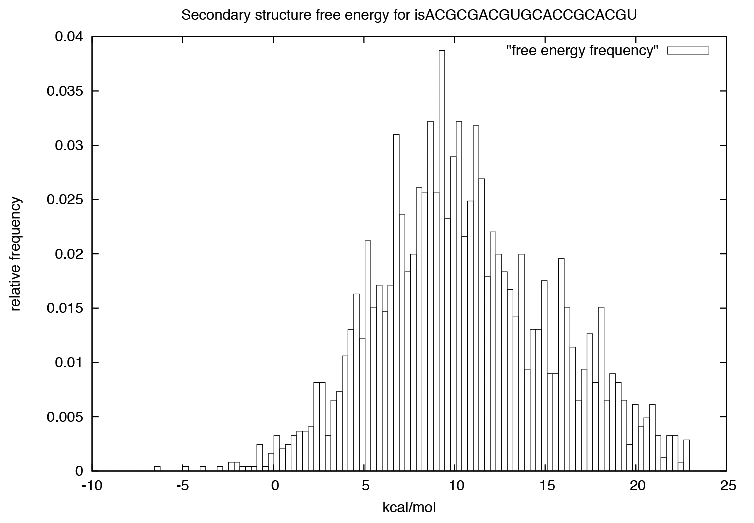
\includegraphics[width=0.525\textwidth]{Figures/Hermes/plmvDist.pdf}
\quad
\includegraphics[width=0.375\textwidth]{Figures/Hermes/plmvStr.pdf}
\caption{
{\em (Left)} Histogram of free energies of secondary structures of
ACGCGACGUGCACCGCACGU, which range from $-6.5$ to $+25$ kcal/mol, with
mean of $10.695$ kcal/mol.
{\em (Right)} Minimum free energy structure of the 54 nt Peach Latent Mosaic
Viroid (PLMVd) AJ005312.1/282-335, which is identical to the consensus
structure from Rfam 11.0 \cite{Gardner.nar11}. \rfold from
Vienna RNA Package 2.1.7 with energy parameters from the Turner 1999
model were used, since the minimum free energy structure determined by
the more recent Turner 2004 energy parameters
does {\em not} agree with the Rfam consensus structure --- see
\cite{syntheticHammerheads}. Positional entropy, a measure
of divergence in the base pairing status at each positions for the
low energy ensemble of structures, is indicated by color, using the
RNA Vienna Package utility script {\tt relplot.pl}.
}
\label{fig:hermes:plmv}
\end{figure}

Figure \ref{fig:hermes:kinfoldMeanStdev} displays the mean
and standard deviation for \kinfold simulations of folding time
for each of the 1,000 RNA sequences from our benchmarking data. For
each sequence, the mean and standard deviation of the time required to
fold the empty structure to the MFE structure were computed from
10,000 \kinfold runs, each run with an upper bound of $10^8$
Monte Carlo steps, thus ensuring that all simulations converged. The
sequences were then sorted by increasing folding time mean. Standard
deviation exceeded the mean in $83.9\%$ of the 1,000 cases, indicating
the enormous variation between separate \kinfold runs, even for
20 nt RNA sequences having at most 2,500 secondary structures. In our
opinion, \kinfold is an expertly crafted implementation of
Gillespie's algorithm for an event driven Monte Carlo simulation of
one-step RNA secondary structure folding. From the standpoint of
biophysics and physical chemistry, there is no more reliable
simulation method, except of course the exact computation of mean
first passage time using linear algebra. Nevertheless, the enormous
time required for reliable \kinfold estimations and the large
standard deviations observed point out the need for a faster method to
approximate folding time.

\begin{figure}
\centering
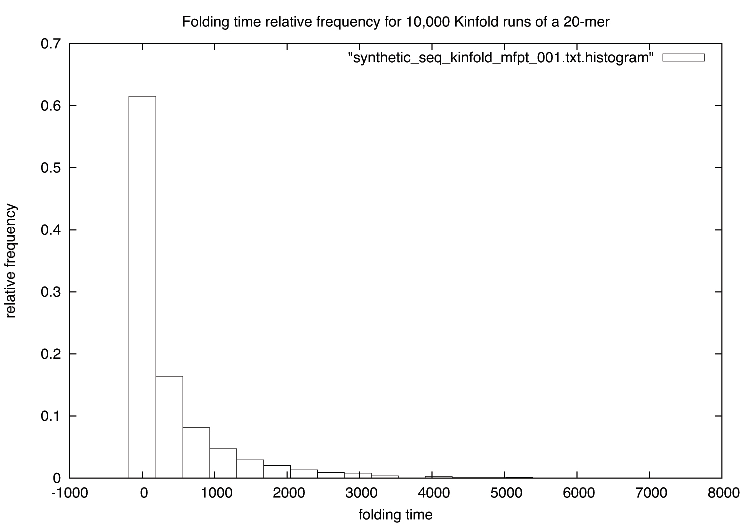
\includegraphics[width=0.45\textwidth]{Figures/Hermes/kinfoldTimeDist.pdf}
\quad
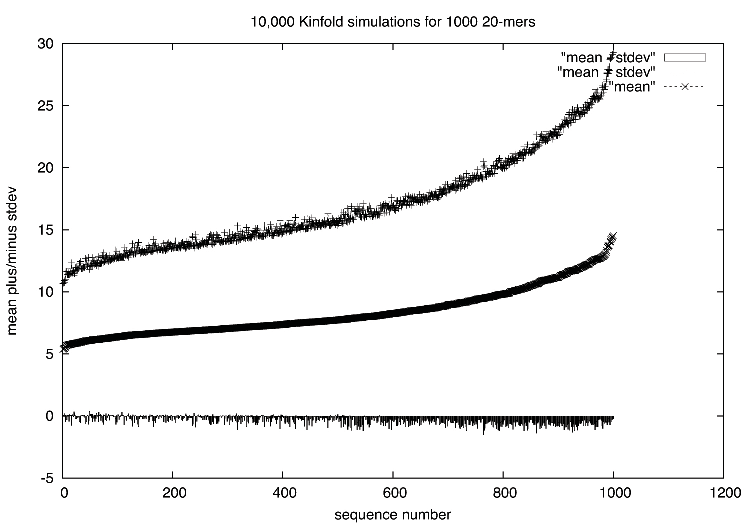
\includegraphics[width=0.45\textwidth]{Figures/Hermes/kinfoldMeanStdev.pdf}
\caption{{\em (Left)} Histogram of \kinfold folding times for 20-mer CCGAUUGGCG AAAGGCCACC. The mean [resp. standard deviation] of 10,000 runs of \kinfold for this 20-mer is 538.37 [resp. 755.65]. Note the close fit to the exponential distribution, {\em (Right)} Mean minus standard deviation ($\mu -\sigma$), mean ($\mu$), and mean plus standard deviation ($\mu + \sigma$) of the logarithm of \kinfold folding times, taken over 10,000 runs for each of the 1,000 sequences from the benchmarking set of 20-mers. For graphical illustration, we have sorted the log folding times in increasing order.}
\label{fig:hermes:kinfoldMeanStdev}
\end{figure}

\subsubsection{Pearson correlation coefficients for various kinetics packages}
\label{subsubsec:hermes:corrtable}

In this section, we display the correlation between (1) the {\em gold
standard} method \rnamfpt, both with and without the Hastings
modification using equations (\ref{eq:hermes:MFPTwithHastings}) and
(\ref{eq:hermes:MFPTwithoutHastings}), (2) the {\em platinum standard} method {\tt
Equilibrium}, (3) the {\em silver standard} method \kinfold, (4) {\tt
FFTmfpt} with and without the Hastings modification using equations
(\ref{eq:hermes:transitionProbabilityFFTbor2DwithHastings}) and
(\ref{eq:hermes:transitionProbabilityFFTbor2DwithoutHastings}), (5) \ffteq
which computes \eqt for the 2D-grid, (6) \rnatwofold
with and without the Hastings modification using equations
(\ref{eq:hermes:transitionProbabilityFFTbor2DwithHastings}) and
(\ref{eq:hermes:transitionProbabilityFFTbor2DwithoutHastings}). Correlations
with [resp. without] the Hastings modification are summarized in the
lower [resp. upper] triangular portion of
Table~\ref{table:correlation}. It is clear that correlations between
the mathematically exact methods \rnamfpt, \rnaeq, and
approximation methods \kinfold, \fftmfpt, \ffteq, \rnatwofold are
improved when using the Hastings correction.

Figures~\ref{fig:hermes:scatterplotRnaEqVsRnaMfptHastingsAndKinfold},
\ref{fig:hermes:scatterplotRnaMfptHastingsVsKinfoldAndFftMfpt},
\ref{fig:hermes:scatterplotFftMfptVsKinfoldAndFftEq}
depict scatterplots for kinetics obtained by some of the algorithms
above. The left panel of
Figure \ref{fig:hermes:scatterplotRnaEqVsRnaMfptHastingsAndKinfold}
shows a scatter plots for gold standard \rnamfpt versus platinum
standard \rnaeq, with correlation value 0.5652. The right
panel of the same figure shows a scatter plot for \kinfold versus
\rnaeq, with correlation 0.7814. Note the persence of two
clusters in this and some of the other scatter plots. Cluster A
consists of RNA sequences whose folding time, as determined by \rnamfpt
or \rnaeq, is rapid --- specifically, the natural
logarithm of the MFPT is at most 7.5. Cluster B consists of the
remaining RNA sequences, whose folding time is longer than that of
cluster A. There are no significant differences between RNA sequences
in clusters A and B with respect to GC-content, sequence logo, minimum
free energy, number of secondary structures, etc.  The left panel of
Figure \ref{fig:hermes:scatterplotRnaMfptHastingsVsKinfoldAndFftMfpt}
shows the scatter plot for \rnamfpt versus \kinfold, with
correlation 0.7933, and the right panel shows the scatter plot for
\rnamfpt versus \fftmfpt, with correlation 0.6035.
Figure \ref{fig:hermes:scatterplotFftMfptVsKinfoldAndFftEq}
shows scatter plots for \fftmfpt versus \kinfold {\em (Left)} and
for \fftmfpt versus \ffteq {\em (Right)}, with respective
correlation values 0.7608 and 0.9589. \kinfold obviously provides
a better correlation with the exact value of \mfpt;
however, since the standard deviation of \kinfold runs is as
large as the mean,\footnote{It follows from spectral decomposition that
\eqt follows an exponential distribution (or sum of
exponential distributions). Exponential distributions have the property
that the mean is equal to the standard deviation, hence
it is not surprising that \kinfold
kinetics have this property.} accurate kinetics estimates
from \kinfold require prohibitively large computational time --- indeed, in
\cite{wolfingerStadler:kinetics} reliable kinetics for phe-tRNA from
yeast were obtained by 9,000 \kinfold simulations, each for $10^8$
steps, requiring 3 months of CPU time on an Intel Pentium 4 running at
2.4 GHz under Linux. Although the correlation value of 0.6035 between
\rnamfpt and \fftmfpt is much less than that obtained by {\tt
Kinfold}, the runtime required by our method \fftmfpt is measured
in seconds, even for moderate to large RNAs. For this reason, we
advocate the use of \fftmfpt in synthetic biology screens to
design RNA sequences having certain desired kinetic properties. Once
promising candidates are found, it is possible to devote additional
computational time to \kinfold simulations for more accurate
kinetics.


\begin{figure}[!h]
\centering
\includegraphics[width=0.45\textwidth]{Figures/Hermes/rnaMfptHastingsRnaEq.pdf}
\quad
\includegraphics[width=0.45\textwidth]{Figures/Hermes/rnaEqKinfold.pdf}
\caption{ Scatter plots of the natural logarithm of times from \rnamfpt
versus \rnaeq {\em (Left)} and for \kinfold versus
\rnaeq {\em (Right)}. }
\label{fig:hermes:scatterplotRnaEqVsRnaMfptHastingsAndKinfold}
\end{figure}


\begin{figure}[!h]
\centering
\includegraphics[width=0.45\textwidth]{Figures/Hermes/rnaMfptHastingsKinfold.pdf}
\quad
\includegraphics[width=0.45\textwidth]{Figures/Hermes/rnaMfptHastingsFftMfptHastings.pdf}
\caption{ Scatter plots of the natural logarithm of times from \rnamfpt
versus \kinfold {\em (Left)} and for \rnamfpt versus {\tt
FFTmfpt} {\em (Right)}. }
\label{fig:hermes:scatterplotRnaMfptHastingsVsKinfoldAndFftMfpt}
\end{figure}


\begin{figure}[!h]
\centering
\includegraphics[width=0.45\textwidth]{Figures/Hermes/kinfoldFftMfptHastings.pdf}
\quad
\includegraphics[width=0.45\textwidth]{Figures/Hermes/fftMfptFftEq.pdf}
\caption{ Scatter plots of the natural logarithm of times from \kinfold
versus \fftmfpt {\em (Left)} and for \fftmfpt versus \ffteq
{\em (Right)}. }
\label{fig:hermes:scatterplotFftMfptVsKinfoldAndFftEq}
\end{figure}

\begin{landscape}
\begin{table}[!h]
\centering
\begin{tabularx}{\linewidth}{c c *{8}{Y}}
  \toprule
  \small{Hastings (Yes\textbackslash No)} & \small{\rnamfpt} & \small{\rnaeq} & \small{\kinfold} & \small{\fftmfpt} & \small{\rnatwofold} & \small{\fftbor} & \small{\ms{BarriersEq}} & \small{\ffteq} \\
  \cmidrule(l){2-9}
  \small{\rnamfpt}   & 1      & 0.5683 & 0.7945 & 0.5060 & 0.5110 & 0.5204 & 0.5280 & 0.4472 \\
  \small{\rnaeq}   & 0.5798 & 1      & 0.7814 & 0.7043 & 0.7025 & 0.5080 & 0.5979 & 0.6820 \\
  \small{\kinfold}       & 0.7933 & 0.7507 & 1      & 0.7312 & 0.7358 & 0.6241 & 0.6328 & 0.6445 \\
  \small{\fftmfpt}       & 0.6035 & 0.7935 & 0.7608 & 1      & 0.9980 & 0.5485 & 0.8614 & 0.9589 \\
  \small{\rnatwofold}     & 0.6076 & 0.7919 & 0.7655 & 0.9983 & 1      & 0.5584 & 0.8538 & 0.9515 \\
  \small{\fftbor}        & 0.5416 & 0.5218 & 0.6241 & 0.5748 & 0.5855 & 1      & 0.3450 & 0.4229 \\
  \small{\ms{BarriersEq}} & 0.6346 & 0.6578 & 0.6328 & 0.8310 & 0.8217 & 0.3450 & 1      & 0.9149 \\
  \small{\ffteq}         & 0.5614 & 0.7916 & 0.6966 & 0.9670 & 0.9590 & 0.4757 & 0.8940 & 1      \\
  \bottomrule
 \end{tabularx}
 \caption{Table of Pearson correlation coefficients for various methods to compute or approximate RNA secondary structure folding kinetics. Lower [resp. upper] triangular entries are with [resp. without] the Hastings correction for Markov chain probability matrices. The methods are: \rnamfpt (\mfpt, computed by matrix inversion for the Markov chain consisting of all secondary structures, with move allowed between structures differing by one base pair), \rnaeq (\eqt, computed by spectral decomposition of a rate matrix comprising all secondary structures to compute population fraction $P(t)$ at time $t$), \kinfold (an implementation of Gillespie's Algorithm to approximate refolding pathways using an event-based Monte Carlo simulation), \fftmfpt (\mfpt for Markov chain consisting of ``grid point'' states $(x,y)$ with probability $P(x,y)=\sum_S exp(-E(S)/RT)/Z$, computed by \ffttwo, where the sum is taken over structures having base pair distance $x$ to the empty structure and $y$ to the MFE structure, \rnatwofold (\mfpt, computed as previously explained, but using \rnatwofold in place of \ffttwo to compute $P(x,y)$), \fftbor (\mfpt, computed for the Markov chain consisting of states $0,1,\dots,n$, for which $P(x) = \sum_S \exp(-E(S)/RT)/Z$, where the sum is taken over all secondary structures whose base pair distance is $x$ from the MFE structure), {\tt BarriersEq} (\eqt, computed using spectral decomposition on the Markov process consisting of ``grid point'' states output from {\tt Barriers}), and \ffteq (\eqt, computed in the same fashion as {\tt BarriersEq} using a Markov process derived from the energy landscape output by \ffttwo). }
\label{table:correlation}
 \end{table}
 \end{landscape}

%!TEX root = ../main.tex

\chapter{Discussion}
\label{ch:disc}

\lhead{Discussion}

Over the course of this thesis, we have described a collection of tools aimed
at facilitating the computational analysis of RNA. The work in \Chref{rfinder}


%----------------------------------------------------------------------------------------
%	THESIS CONTENT - APPENDICES
%----------------------------------------------------------------------------------------
% \addtocontents{toc}{\vspace{2em}} % Add a gap in the Contents, for aesthetics

\appendix % Cue to tell LaTeX that the following 'chapters' are Appendices

%!TEX root = ../main.tex

\chapter{FFTbor Appendix}
\label{ch:fftborapp}

\lhead{FFTbor Appendix}

\section{Full recursions for \texorpdfstring{\emZ{i,j}}{}
for the Turner energy model}
\label{sec:fftbor:turner}

To compute $\emZ{} = \emZ{1,n}$ given input structure \str, we use the recursions

\begin{align}
\label{eq:fftborapp:zx}
\emZ{i,j} = \emZ{i,j-1} \cdot x^{d_0} +
\sum_{\mathclap{\substack{(s_k,s_j) \in \bpSet, \\ i \leq k < j}}}\enspace
\Big( \emZ{i,k-1} \cdot \emZB{k,j} \cdot \boltzE{E_d} \cdot x^{d_1} \Big),
\end{align}

where $d_0 = 1$ if $j$ is base paired
in $\str_{[i,j]}$ and $0$ otherwise, $d_1 =
\dBP{\str_{[i,j]}}{\str_{[i,k-1]} \cup \str_{[k,j]}}$, and $E_d$
is the energy contribution due to dangling ends (energy
contributions from single bases stacking on adjacent base pairs) and
closing AU base pairs (since a non GC base pair closing a stem has a
destabilizing effect).  The sum is taken over all possible
base pairs $(k,j)$ with $i \leq k < j$.

We compute \emZB{} using the recursion

\begin{align}
\label{eq:fftborapp:zbx}
\begin{split}
\emZB{i,j} &= \boltzE{EH(i,j)} \cdot x^{d_2} \\
&+ \sum_{\mathclap{\substack{(s_k,s_l) \in \bpSet, \\ i < k < l < j }}}\enspace
\emZB{k,l} \cdot \boltzE{EI(i,j,k,l)} \cdot x^{d_3} \\
&+ \sum_{\mathclap{\substack{(s_k,s_l) \in \bpSet, \\ i < k < l < j }}}\enspace
\Big( \emZM{i+1,k-1} \cdot \emZB{k,l} \cdot \boltzE{(a+b+c(j-l-1))}
\cdot x^{d_4} \Big)
\end{split}
\end{align}

where $d_2 = \dBP{\str_{[i,j]}}{\{(i,j)\}}$,
$EH(i,j)$ is the energy of the hairpin loop with closing base
pair $(i,j)$, $EI(i,j,k,l)$ is the energy of the stack, bulge or
interior loop with the closing base pair $(i,j)$ and the interior
base pair $(k,l)$, $d_3 = \dBP{\str_{[i,j]}}{\str_{[k,l]} \cup
\{(i,j)\}}$, and $d_4 = \dBP{\str_{[i,j]}}{\str_{[i+1,k-1]} \cup
\str_{[k,l]} \cup\{(i,j)\}}$. The first term in the
recursion takes care of the case where $(i,j)$ is the only base pair
in $[i,j]$, i.e. $(i,j)$ closes a hairpin loop. The second term
handles the case where there is an interior loop (or a bulge or a
stack) closed by $(i,j)$ and $(k,l)$. The third term takes care of
all the structures where $(i,j)$ closes a multiloop. To reduce
complexity of the algorithm, the interior and bulge loop size can be
limited to a maximum size of $L$ (taken by default to be $30$),
by requiring that $l>j-L$ in the above recursion.

The final recursion, for computing \emZM{}, is

\begin{align}
\label{eq:fftborapp:zmx}
\begin{split}
\emZM{i,j} &= \emZM{i,j-1} \cdot \boltzE{c} \cdot x^{d_0} \\
&+ \sum_{\mathclap{\substack{(s_k,s_j) \in \bpSet, \\ i \leq k < j }}}\enspace
\Big( \emZB{k,j} \cdot \boltzE{(b+c(k-i))} \cdot x^{d_5} \\
&+ \emZM{i,k-1} \cdot \emZB{k,j} \cdot \boltzE{b} \cdot x^{d_6} \Big)
\end{split}
\end{align}

where $d_5 = \dBP{\str_{[i,j]}}{\str_{[k,j]}}$ and $d_6
=\dBP{\str_{[i,j]}}{\str_{[i,k-1]} \cup \str_{[k,j]}}$.
Note that since $\emZM{i,j}$ computes the partition function
contribution under the assumption that $[i,j]$ is part of a
multiloop, there will be exactly one stem-loop structure in this
region (the \emZB{} term) or
more than one (the \emZM{}--\emZB{} term).
Justification of recursions (\ref{eq:fftborapp:zx}),
(\ref{eq:fftborapp:zbx}), and
(\ref{eq:fftborapp:zmx})
follow by induction, as in the proof of Theorem \ref{thm:fftbor:recursions}.

%!TEX root = ../main.tex

\chapter{FFTbor2D Appendix}
\label{ch:ffttwoapp}

\lhead{FFTbor\twoD Appendix}

\section{Full recursions for \texorpdfstring{\emZ{i,j}}{}
for the Turner energy model}
\label{sec:ffttwo:turner}

To compute $\emZ{} = \emZ{1,n}$ given input structures \strAB,
we use the recursions

\begin{align}
\label{eq:ffttwoapp:zx}
\emZ{i,j} = \emZ{i,j-1} \cdot x^{\ab{0}} +
\sum_{\mathclap{\substack{(s_k,s_j) \in \bpSet, \\ i \leq k < j}}}\enspace
\Big( \emZ{i,k-1} \cdot \emZB{k,j} \cdot \boltzE{E_d} \cdot
x^{\ab{1}} \Big),
\end{align}

where
$\alpha_0 = 1$ if $j$ is base paired in $\strA_{[i,j]}$ and $0$ otherwise,
$\beta_0 = 1$ if $j$ is base paired in $\strB_{[i,j]}$ and $0$ otherwise,
$\alpha_1 = \dBP{\strA_{[i,j]}}{\strA_{[i,k-1]} \cup \strA_{[k,j]}}$,
$\beta_1 = \dBP{\strB_{[i,j]}}{\strB_{[i,k-1]} \cup \strB_{[k,j]}}$,
and $E_d$ is the energy contribution due to dangling ends (energy
contributions from single bases stacking on adjacent base pairs) and
closing AU base pairs (since a non GC base pair closing a stem has a
destabilizing effect).  The sum is taken over all possible
base pairs $(k,j)$ with $i \leq k < j$.

We compute \emZB{} using the recursion

\begin{align}
\label{eq:ffttwoapp:zbx}
\begin{split}
\emZB{i,j} &= \boltzE{EH(i,j)} \cdot x^{\ab{2}} \\
&+ \sum_{\mathclap{\substack{(s_k,s_l) \in \bpSet, \\ i < k < l < j }}}\enspace
\emZB{k,l} \cdot \boltzE{EI(i,j,k,l)} \cdot x^{\ab{3}} \\
&+ \sum_{\mathclap{\substack{(s_k,s_l) \in \bpSet, \\ i < k < l < j }}}\enspace
\Big( \emZM{i+1,k-1} \cdot \emZB{k,l} \cdot \boltzE{(a+b+c(j-l-1))}
\cdot x^{\ab{4}} \Big)
\end{split}
\end{align}

where
$EH(i,j)$ is the energy of the hairpin loop with closing base pair $(i,j)$,
$\alpha_2 = \dBP{\strA_{[i,j]}}{\{(i,j)\}}$,
$\beta_2 = \dBP{\strB_{[i,j]}}{\{(i,j)\}}$,
$EI(i,j,k,l)$ is the energy of the stack, bulge or
interior loop with the closing base pair $(i,j)$ and the interior
base pair $(k,l)$,
$\alpha_3 = \dBP{\strA_{[i,j]}}{\strA_{[k,l]} \cup \{(i,j)\}}$,
$\beta_3 = \dBP{\strB_{[i,j]}}{\strB_{[k,l]} \cup \{(i,j)\}}$,
$\alpha_4 = \dBP{\strA_{[i,j]}}{\strA_{[i+1,k-1]} \cup
\strA_{[k,l]} \cup\{(i,j)\}}$, and
$\beta_4 = \dBP{\strB_{[i,j]}}{\strB_{[i+1,k-1]} \cup
\strB_{[k,l]} \cup\{(i,j)\}}$.
The first term in the
recursion takes care of the case where $(i,j)$ is the only base pair
in $[i,j]$, i.e. $(i,j)$ closes a hairpin loop. The second term
handles the case where there is an interior loop (or a bulge or a
stack) closed by $(i,j)$ and $(k,l)$. The third term takes care of
all the structures where $(i,j)$ closes a multiloop. To reduce
complexity of the algorithm, the interior and bulge loop size can be
limited to a maximum size of $L$ (taken by default to be $30$),
by requiring that $l>j-L$ in the above recursion.

The final recursion, for computing \emZM{}, is

\begin{align}
\label{eq:ffttwoapp:zmx}
\begin{split}
\emZM{i,j} &= \emZM{i,j-1} \cdot \boltzE{c} \cdot x^{\ab{0}} \\
&+ \sum_{\mathclap{\substack{(s_k,s_j) \in \bpSet, \\ i \leq k < j }}}\enspace
\Big( \emZB{k,j} \cdot \boltzE{(b+c(k-i))} \cdot x^{\ab{5}} \\
&+ \emZM{i,k-1} \cdot \emZB{k,j} \cdot \boltzE{b} \cdot x^{\ab{6}} \Big)
\end{split}
\end{align}

where
$\alpha_5 = \dBP{\strA_{[i,j]}}{\strA_{[k,j]}}$,
$\beta_5 = \dBP{\strB_{[i,j]}}{\strB_{[k,j]}}$,
$\alpha_6 =\dBP{\strA_{[i,j]}}{\strA_{[i,k-1]} \cup \strA_{[k,j]}}$, and
$\beta_6 =\dBP{\strB_{[i,j]}}{\strB_{[i,k-1]} \cup \strB_{[k,j]}}$.
Note that since $\emZM{i,j}$ computes the partition function
contribution under the assumption that $[i,j]$ is part of a
multiloop, there will be exactly one stem-loop structure in this
region (the \emZB{} term) or
more than one (the \emZM{}--\emZB{} term).
Justification of recursions (\ref{eq:ffttwoapp:zx}),
(\ref{eq:ffttwoapp:zbx}), and
(\ref{eq:ffttwoapp:zmx})
follow by induction, as in the proof of Theorem \ref{thm:ffttwo:recursions}.

\section{Proof for Theorem \ref{thm:ffttwo:recursions}}
\label{sec:ffttwo:recursions}

\begin{proof}
Recall that if $F$ is an arbitrary
polynomial [resp. analytic] function, then $[x^{rn+s}]F(x)$
denotes the coefficient of monomial $x^{rn+s}$ in the
Taylor expansion of $F(x)$. For instance, in
\eqnref{ffttwo:pOfX}, $[x^{rn+s}]p(x) = p_{rn+s}$, and in
\eqnref{ffttwo:zOfX}, $[x^{rn+s}]\fullZx = z_{rn+s}$.

By definition, it is clear that $\emZ{i,j}=1$ if $i \leq j \leq i + \theta$,
where we recall that $\theta = 3$ is the minimum number of unpaired bases in
a hairpin loop. For $j > i + \theta$, we have

\begin{align}
\begin{split}
[x^{rn+s}] \emZ{i,j} &= z_{rn+s}(i,j) = \bfZ{rn+s}{i,j} \\
&= \bfZ{(r-\alpha_0)n+(s-\beta_0)}{i,j-1} \\
&+
\sum_{k=i}^{j-1}\enspace
\sum_{u_0+u_1=r-\alpha(k)}\enspace
\sum_{v_0+v_1=s-\beta(k)}
\left( \boltzNuss{k,j}
\cdot \bfZ{u_0 n+v_0}{i,k-1} \cdot \bfZ{u_1 n+v_1}{k+1,j-1} \right) \\
&= [x^{(r-\alpha_0)n+(s-\beta_0)}] \emZ{i,j-1} \\
&+ \sum_{k=i}^{j-1}\enspace
\sum_{u_0+u_1=r-\alpha(k)}\enspace
\sum_{v_0+v_1=s-\beta(k)}
\left( \boltzNuss{k,j} \right. \\
&\left. \cdot \left( [x^{u_0 n+v_0}] \emZ{i,k-1} \right) \cdot
\left( [x^{u_1 n+v_1}] \emZ{k+1,j-1} \right)
\vphantom{\boltzNuss{k,j}} \right) \\
&= [x^{(r-\alpha_0)n+(s-\beta_0)}] \emZ{i,j-1} \\
&+ \sum_{k=i}^{j-1}\enspace
\sum_{u_0+u_1=r-\alpha(k)}\enspace
\sum_{v_0+v_1=s-\beta(k)}
\left( \boltzNuss{k,j} \right. \\
&\left. \cdot [x^{(u_0+u_1)n+(v_0+v_1)}] \left( \emZ{i,k-1} \cdot \emZ{k+1,j-1} \right)
\vphantom{\boltzNuss{k,j}} \right) \\
&= [x^{(r-\alpha_0)n+(s-\beta_0)}] \emZ{i,j-1} \\
&+ \sum_{k=i}^{j-1} \left( \boltzNuss{k,j}
\cdot [x^{(r-\alpha(k))n+(s-\beta(k))}] \left( \emZ{i,k-1} \cdot \emZ{k+1,j-1}
\right) \right) \\
&= [x^{rn+s}] \left( \emZ{i,j-1} \cdot x^{\ab{0}} \right) \\
&+ \sum_{k=i}^{j-1} \left( \boltzNuss{k,j}
\cdot [x^{rn+s}] \left( \emZ{i,k-1} \cdot \emZ{k+1,j-1} \cdot
x^{\alpha(k)n+\beta(k)} \right) \right) \\
&= [x^{rn+s}] \left( \vphantom{\sum_{k=i}^{j-1}} \emZ{i,j-1} \cdot x^{\ab{0}} \right. \\
&\left. + \sum_{k=i}^{j-1} \left( \boltzNuss{k,j}
\cdot \emZ{i,k-1} \cdot \emZ{k+1,j-1} \cdot
x^{\alpha(k)n+\beta(k)} \right) \right) \\
\end{split}
\end{align}
\end{proof}

\section{Proof for Lemma \ref{lem:ffttwo:lemma3}}
\label{sec:ffttwo:lemma3proof}

\begin{proof}
The lemma states that if the \bpd $d_0$ between reference
structures \strAB is even, then $\emZof{}{-\alpha}=\emZof{}{\alpha}$, while if
the distance is odd, then $\emZof{}{-\alpha}=-\emZof{}{\alpha}$.
Suppose first that $d_0$ is even. By Lemma \ref{lem:ffttwo:lemma1},
$\emZ{} = z_0 + z_2 x^2 + z_4 x^4 + \dots +
z_{M-2} x^{M-2)}$, and so $\emZof{}{-\alpha}=\emZof{}{\alpha}$.
Suppose now that
$d_0$ is odd. By Lemma \ref{lem:ffttwo:lemma1},
$Z(x) = z_1 x^1 + z_3 x^3 + z^5 x^5 \dots +
z_{M-1} x^{M-1}$, and so $\emZof{}{-\alpha}=-\emZof{}{\alpha}$.
\end{proof}

\section{Proof for Lemma \ref{lem:ffttwo:lemma4}}
\label{sec:ffttwo:lemma4proof}

\begin{proof}
Recall Euler's formula in complex analysis:
$\exp(ix) = \cos(x) + i \sin(x)$. As well, recall that
$\sin(\pi)=0$, $\cos(\pi)=-1$, and the trigonometric
addition formulas:

\begin{align}
\begin{split}
\cos(\alpha-\beta) &= \cos(\alpha) \cos(\beta) + \sin(\alpha) \sin(\beta) \\
\sin(\alpha-\beta) &= \sin(\alpha) \cos(\beta) - \sin(\beta) \cos(\alpha).
\end{split}
\end{align}

Then we have

\begin{align}
\begin{split}
\nu^{M_0-k} &= \exp\left(\frac{2 \pi i (M_0-k)}{M}\right) \\
&= \cos\left(\frac{2 \pi (M_0-k)}{M}\right) + i
\sin\left(\frac{2 \pi (M_0-k)}{M}\right) \\
&= \cos\left(\pi - \frac{2 \pi k}{M}\right) + i
\sin\left(\pi - \frac{2 \pi k}{M}\right) \\
&=
\left[
\cos(\pi) \cos\left(\frac{2 \pi k}{M}\right) +
\sin(\pi) \sin\left(\frac{2 \pi k}{M}\right)
\right] \\
&+
i \left[
\sin(\pi) \cos\left(\frac{2 \pi k}{M}\right) -
\sin\left(\frac{2 \pi k}{M}\right) \cos(\pi)
\right] \\
&=
-\cos\left(\frac{2 \pi k}{M}\right) + i
\sin\left(\frac{2 \pi k}{M}\right) \\
&=
-1 \left[ \cos\left(\frac{2 \pi k}{M}\right) - i
\sin\left(\frac{2 \pi k}{M}\right) \right] \\
&=
-1 \cdot \overline{\cos\left(\frac{2 \pi k}{M}\right) + i
\sin\left(\frac{2 \pi k}{M}\right)}  \\
&=
-1 \cdot \overline{\exp\left(\frac{2 \pi i k}{M}\right)} = - \overline{\nu^k} . \\
\end{split}
\end{align}

It follows that
$\nu^{M_0-k} = -\overline{\nu^k}$, so
$\nu^{k} = \overline{- \nu^{(M_0-k)}} = -\overline{\nu^{(M_0-k)}}$.

This completes the proof of the lemma.
\end{proof}


% \addtocontents{toc}{\vspace{2em}} % Add a gap in the Contents, for aesthetics

\backmatter

%----------------------------------------------------------------------------------------
%	BIBLIOGRAPHY
%----------------------------------------------------------------------------------------
\label{Bibliography}

\setstretch{1.3}

\lhead{\emph{Bibliography}}

\bibliographystyle{ieeetr}

\bibliography{Biblio/Full}

\end{document}
